\documentclass[12pt,a4paper]{article}
\usepackage[a4paper, margin=0.8in, headheight=14pt]{geometry}
\usepackage{fontspec}
\usepackage{unicode-math}
\setmainfont{TeX Gyre Pagella}
\setmonofont[Scale=0.88]{TeX Gyre Cursor}
\setmathfont{Latin Modern Math}
\usepackage{xcolor}
\usepackage{colortbl}
\usepackage{titlesec}
\usepackage{enumitem}
\usepackage{tabularx}
\usepackage{booktabs}
\usepackage{array}
\usepackage{amsmath}
\allowdisplaybreaks
\usepackage{tikz}
\usetikzlibrary{shapes.geometric, arrows.meta, positioning, calc, fit, decorations.pathreplacing, decorations.pathmorphing, patterns, backgrounds}
% circuitikz not required for this subject
\usepackage{tcolorbox}
\tcbuselibrary{skins, breakable}
\usepackage{etoolbox}
\usepackage{hyperref}
\usepackage{fancyhdr}
\usepackage{graphicx}
\usepackage{microtype}
\hyphenpenalty=10000
\exhyphenpenalty=10000
\sloppy
\usepackage{caption}
\usepackage{setspace}
\usepackage{multirow}
\usepackage{tocloft}
\newcommand{\Q}[1]{\textbf{#1}\par\noindent\ignorespaces}
\definecolor{myred}{RGB}{196,30,58}
\definecolor{mydark}{RGB}{30,30,50}
\definecolor{mygreen}{RGB}{14,120,80}
\definecolor{myteal}{RGB}{0,130,140}
\definecolor{myamber}{RGB}{180,100,0}
\definecolor{mypurple}{RGB}{100,30,160}
\definecolor{mygray}{RGB}{246,247,249}
\definecolor{mgframe}{RGB}{180,185,200}
\definecolor{watermark}{RGB}{145,150,170}
\definecolor{hdrred}{RGB}{250,232,235}
\definecolor{hdrgreen}{RGB}{220,244,233}
\definecolor{hdrteal}{RGB}{220,242,244}
\definecolor{hdramber}{RGB}{253,242,215}
\definecolor{hdrpurple}{RGB}{238,228,255}
\definecolor{hdrgray}{RGB}{238,240,245}
\AfterEndEnvironment{tcolorbox}{\color{mydark}}

\titleformat{\section}{\large\bfseries\color{myred}}{\thesection.}{0.5em}{}[\vspace{1pt}{\color{myred}\rule{\linewidth}{0.8pt}}]
\titleformat{\subsection}{\normalsize\bfseries\color{myteal}}{\thesubsection}{0.5em}{}
\titlespacing*{\section}{0pt}{18pt}{7pt}
\titlespacing*{\subsection}{0pt}{11pt}{4pt}
\setlength{\parindent}{0pt}
\setlength{\parskip}{4pt}
\renewcommand{\cfttoctitlefont}{\large\bfseries\color{myred}}
\renewcommand{\cftaftertoctitle}{\par\noindent{\color{myred}\rule{\linewidth}{0.8pt}}}
\setlength{\cftbeforetoctitleskip}{0pt}
\setlength{\cftaftertoctitleskip}{6pt}
\renewcommand{\cftsecfont}{\normalsize\bfseries\color{mydark}}
\renewcommand{\cftsecpagefont}{\normalsize\bfseries\color{mydark}}
\renewcommand{\cftsecleader}{\cftdotfill{\cftdotsep}}
\setlength{\cftbeforesecskip}{5pt}
\renewcommand{\cftsubsecfont}{\small\color{mydark}}
\renewcommand{\cftsubsecpagefont}{\small\color{mydark}}
\setlength{\cftbeforesubsecskip}{2pt}
\setlength{\cftsubsecindent}{1.4em}
\renewcommand{\cftpartfont}{\normalsize\bfseries\color{myteal}}
\renewcommand{\cftpartpagefont}{\normalsize\bfseries\color{myteal}}
\setlength{\cftbeforepartskip}{10pt}
\renewcommand{\arraystretch}{1.45}
\setlength{\tabcolsep}{6pt}
\arrayrulecolor{mydark}
\newcolumntype{B}[1]{>{\small\bfseries\raggedright\arraybackslash}m{#1}}
\newcolumntype{C}[1]{>{\centering\arraybackslash}m{#1}}
\newcolumntype{Y}{>{\small\raggedright\arraybackslash}X}
\renewcommand{\tabularxcolumn}[1]{m{#1}}
\newcommand{\currmodule}{Module 1}
\pagestyle{fancy}
\fancyhf{}
\fancyhead[L]{\small\color{myred}\textbf{ES-CS401}\;\color{mydark}--- Design and Analysis of Algorithms}
\fancyhead[R]{\small\color{myteal}\textbf{\currmodule\ Notes}}
\fancyfoot[C]{\small\color{mydark}\thepage}
\fancyfoot[R]{\small\color{watermark}\textit{\copyright\ Biraj}}
\renewcommand{\headrulewidth}{0.5pt}
\renewcommand{\footrulewidth}{0.3pt}

\hypersetup{colorlinks=true, linkcolor=myteal, urlcolor=myteal,
  pdfauthor={Biraj Sarkar},
  pdftitle={ES-CS401 --- Combined Notes}}

\tcbset{
  tikzbox/.style={
    colback=mygray, colframe=mgframe, boxrule=0.6pt, arc=4pt,
    left=8pt, right=8pt, top=6pt, bottom=6pt,
    colbacktitle=mgframe, coltitle=mydark, fonttitle=\small\bfseries
  },
  defbox/.style={
    colback=hdrgreen, colframe=mygreen, boxrule=0.8pt, arc=4pt,
    left=9pt, right=9pt, top=6pt, bottom=6pt,
    colbacktitle=mygreen, coltitle=white, fonttitle=\small\bfseries
  },
  formulabox/.style={
    colback=hdrteal, colframe=myteal, boxrule=0.8pt, arc=4pt,
    left=9pt, right=9pt, top=7pt, bottom=7pt,
    colbacktitle=myteal, coltitle=white, fonttitle=\small\bfseries
  },
  examplebox/.style={
    colback=hdramber, colframe=myamber, boxrule=0.8pt, arc=4pt,
    left=9pt, right=9pt, top=6pt, bottom=6pt,
    colbacktitle=myamber, coltitle=white, fonttitle=\small\bfseries
  },
  masonbox/.style={
    colback=hdrpurple, colframe=mypurple, boxrule=0.8pt, arc=4pt,
    left=9pt, right=9pt, top=6pt, bottom=6pt,
    colbacktitle=mypurple, coltitle=white, fonttitle=\small\bfseries
  },
  exambox/.style={
    colback=hdrpurple, colframe=mypurple, boxrule=1pt, arc=5pt,
    left=10pt, right=10pt, top=8pt, bottom=8pt,
    colbacktitle=mypurple, coltitle=white, fonttitle=\bfseries,
    breakable, title after break={\textbf{Frequently Asked / Viva Questions (contd.)}}
  }
}
\tcbset{breakable}
\tcbset{coltext=mydark}
\tcbset{after={\color{mydark}}}

\tikzset{
  block/.style={rectangle, draw=myteal, fill=hdrteal,
    text width=2.4cm, align=center, minimum height=0.95cm,
    font=\small, rounded corners=3pt, line width=0.7pt},
  redblock/.style={rectangle, draw=myred, fill=hdrred,
    text width=2.4cm, align=center, minimum height=0.95cm,
    font=\small, rounded corners=3pt, line width=0.7pt},
  amberblock/.style={rectangle, draw=myamber, fill=hdramber,
    text width=2.4cm, align=center, minimum height=0.95cm,
    font=\small, rounded corners=3pt, line width=0.7pt},
  sumjunc/.style={circle, draw=myamber, fill=hdramber,
    minimum size=0.62cm, font=\small, line width=0.8pt},
  arrow/.style={-Stealth, thick, color=mydark},
  redarrow/.style={-Stealth, thick, color=myred},
  line/.style={thick, color=mydark}
}

\newcommand{\modulestart}[2]{%
  \clearpage
  \renewcommand{\currmodule}{Module #1}%
  \renewcommand{\theHsection}{mod#1.\arabic{section}}%
  \renewcommand{\theHsubsection}{\theHsection.\arabic{subsection}}%
  \renewcommand{\theHsubsubsection}{\theHsubsection.\arabic{subsubsection}}%
  \phantomsection
  \addcontentsline{toc}{part}{Module #1: #2}%
  \setcounter{section}{0}%
  \begin{center}
    \vspace*{1.0cm}
    {\Huge\bfseries\color{myred} Module #1}\\[10pt]
    {\Large\bfseries\color{mydark} #2}\\[10pt]
    {\color{myred}\rule{0.55\linewidth}{1.2pt}}
  \end{center}
  \vspace{14pt}
}
\begin{document}

\thispagestyle{empty}

% ─── Page Border (TikZ Overlay) ────────────────────────────────────────────────
\begin{tikzpicture}[remember picture, overlay]
  % Outer border (fine line in mgframe)
  \draw[color=mgframe, line width=1.5pt] 
    ($(current page.north west) + (0.6in, -0.6in)$) rectangle 
    ($(current page.south east) + (-0.6in, 0.6in)$);
  % Inner border (finer accent line in myred)
  \draw[color=myred, line width=0.8pt] 
    ($(current page.north west) + (0.65in, -0.65in)$) rectangle 
    ($(current page.south east) + (-0.65in, 0.65in)$);
\end{tikzpicture}

\vspace*{1.0cm}
\begin{center}
  {\Huge\bfseries\color{myred} ES-CS401}\\[10pt]
  {\LARGE\bfseries\color{mydark} Design and Analysis of Algorithms}\\[20pt]
  {\color{myred}\rule{0.7\linewidth}{1.5pt}}\\[18pt]
  {\Large\color{myteal}\textbf{Combined Module Notes}}\\[8pt]
  {\large\color{mydark} Modules 1 -- 5}\\[40pt]
  {\normalsize\color{mydark} Semester IV \quad$\bullet$\quad ECE \quad$\bullet$\quad 3 Credits}\\[12pt]
  {\normalsize\color{mydark} CGEC \;$|$\; B.Tech ECE (2023--27)}
\end{center}
\vspace{1.0cm}
\begin{center}
  \begin{tcolorbox}[colback=mygray, colframe=mgframe, boxrule=0.5pt, arc=3pt, width=0.85\linewidth]
    \centering\small\color{mydark}
    \textbf{Disclaimer / Study Guide Notice:}\\
    These are condensed \textbf{Short Notes} focusing on core theory, key formulas, block/circuit diagrams, and standard viva Q\&As for university exam revision. Exhaustive numerical practice problems and derivation edge cases are not covered. This serves as a quick-revision reference guide for students.
  \end{tcolorbox}
\end{center}
\vfill
\vspace{0.6cm}
\begin{center}
  {\large\bfseries\color{mypurple} Biraj Sarkar}\\[16pt]
  {\footnotesize\color{watermark}\textbf{IN ASSOCIATION WITH}}\\[8pt]
  {\small\bfseries\color{mydark} MAKAUT Wingman \quad$\bullet$\quad MAKAUT Future Minds}\\[12pt]
  {\large\bfseries\color{myteal} Cooch Behar Government Engineering College}
\end{center}
\vfill
\begin{center}{\small\color{watermark}\textit{Exam-Ready Notes}}\end{center}
\clearpage

\hypersetup{linkcolor=mydark}
\tableofcontents
\hypersetup{linkcolor=myteal}
\clearpage

% -- Module 1 -----------------------------------------------------------------
\modulestart{1}{Algorithm Analysis and Recurrence Relations}

\section{Algorithm Analysis and Recurrence Relations}
\subsection{Meaning and characteristics of an algorithm}
\begin{tcolorbox}[defbox, title={Algorithm}]
An \textbf{algorithm} is a finite, unambiguous sequence of effective steps that transforms admissible input into the output specified by a problem. A program is an implementation of those steps in a particular language.
\end{tcolorbox}

\begin{itemize}[leftmargin=*, itemsep=3pt, topsep=4pt]
  \item \textbf{Input.} State the admissible data, its range and representation. Some algorithms have no external input.
  \item \textbf{Output.} Specify the answer or effect required for each admissible input.
  \item \textbf{Definiteness.} Each instruction has a precise meaning. A randomized algorithm can still specify exactly how to make a random choice.
  \item \textbf{Finiteness.} A terminating algorithm finishes after finitely many steps on every allowed input.
  \item \textbf{Effectiveness.} Each primitive step is executable with the available operations.
  \item \textbf{Correctness and generality.} The stated result must hold over the entire input domain. A few successful tests only check the selected cases.
\end{itemize}
\textbf{Example specification.} Searching an array takes a sequence $A$ and a key $x$. Return any index containing $x$, or return failure exactly when $x$ is absent. If the required output is the \emph{first} index, that condition belongs in the specification.

\subsection{Correctness proofs and termination}
\begin{tcolorbox}[defbox, title={Loop invariant}]
A \textbf{loop invariant} is a property true just before each iteration. To prove partial correctness, show it holds initially, survives an iteration and implies the desired result when the loop exits. Pair this with a termination argument for total correctness.
\end{tcolorbox}

\begin{tcolorbox}[formulabox, title={Linear search for the first occurrence}]
\begin{verbatim}
FirstIndex(A, x):
    for i = 0, 1, ..., length(A)-1:
        if A[i] == x:
            return i
    return NOT_FOUND
\end{verbatim}
\end{tcolorbox}

\begin{tcolorbox}[examplebox, title={Proving linear search correct}]
\begin{enumerate}[leftmargin=*, itemsep=3pt, topsep=4pt]
  \item \textbf{Initialise.} Before inspecting position $0$, the prefix $A[0..-1]$ is empty and contains no occurrence.
  \item \textbf{Maintain.} If $A[i]=x$, the invariant guarantees no earlier match. Otherwise the inspected prefix can be extended through $i$ and still contains no match.
  \item \textbf{Use the exit condition.} If the loop runs out of positions, the inspected prefix is the entire array, so failure is correct.
  \item \textbf{Prove termination.} The number of unchecked entries falls by one on each iteration that continues. It starts finite and cannot fall below zero.
\end{enumerate}
\end{tcolorbox}

A recursive proof uses the same separation. Check the base case, assume smaller calls satisfy their specifications and show that the returned results combine to satisfy the current specification. Also identify a strictly decreasing non-negative measure, such as subarray length.

\section{Performance Measurement and Asymptotic Bounds}
\subsection{Cost model, input size and experiments}
\begin{enumerate}[leftmargin=*, itemsep=3pt, topsep=4pt]
  \item \textbf{Choose the input-size measure.} Use the number of stored keys for sorting, $V$ and $E$ for graphs, and bit length for encoded integers. An integer of value $W$ uses $\Theta(\log(W+1))$ bits.
  \item \textbf{Specify the model.} In the unit-cost RAM model, operations on fixed-size machine words and direct array access cost constant time. Very large integer multiplication requires a separate bit-cost model.
  \item \textbf{Count a relevant operation.} Comparisons may dominate sorting, edge inspections may dominate traversal, and page reads may dominate an external-memory search.
  \item \textbf{State the case and space convention.} Separate running time from peak auxiliary memory, and state whether input or output storage is included. A recursive call stack counts as auxiliary space.
\end{enumerate}
\textbf{Empirical measurement.} Benchmark different sizes and input families under the same environment. Record elapsed time, operation counts or peak memory. Repeat trials, control warm-up and report variation. This compares implementations and constants. A growth bound over all admissible sizes needs an analytical argument.
\begin{tcolorbox}[examplebox, title={Predicting growth from the model}]
If an implementation takes $2$ ms at $n=1{,}000$ and its dominant work is quadratic, then doubling $n$ predicts about $2(2)^2=8$ ms under comparable conditions. Cache effects and input distribution can change the observed ratio.
\end{tcolorbox}

\subsection{Best, average and worst cases}
Let $\mathcal{I}_n$ be the set of inputs of size $n$ and $C(I)$ the operation count on input $I$.
\begin{tcolorbox}[formulabox, title={Case definitions}]
\begin{align*}
T_{\mathrm{best}}(n)&=\min_{I\in\mathcal{I}_n} C(I),\\
T_{\mathrm{worst}}(n)&=\max_{I\in\mathcal{I}_n} C(I),\\
T_{\mathrm{avg}}(n)&=\sum_{I\in\mathcal{I}_n}\Pr(I)\,C(I).
\end{align*}
The average is relative to a stated input distribution. Expected time over a program's random choices is a separate notion.
\end{tcolorbox}

\begin{tcolorbox}[examplebox, title={Linear search with successful and unsuccessful queries}]
For an array of $n\ge 1$ items, the best successful query compares once and the worst query compares $n$ times. If the target occurs once and its index is uniform,
\begin{align*}
\mathbb{E}[C\mid\text{success}]
  &= \frac{1}{n}\sum_{j=1}^{n}j\\
  &= \frac{n+1}{2}.
\end{align*}
If a query is unsuccessful with probability $q$, it uses all $n$ comparisons on those runs. Under the same uniform-position assumption for successes,
\[
\mathbb{E}[C]=qn+(1-q)\frac{n+1}{2}=\Theta(n).
\]
The best, worst and average are therefore $\Theta(1)$, $\Theta(n)$ and $\Theta(n)$ under these conditions.
\end{tcolorbox}

\subsection{Big-O, Big-Omega and Big-Theta}
\begin{tcolorbox}[defbox, title={Growth bounds}]
For eventually non-negative functions, $f\in O(g)$ means that $f(n)\le c g(n)$ for all $n\ge n_0$ for some $c>0$. The notation $f\in\Omega(g)$ reverses the inequality. The notation $f\in\Theta(g)$ means that both bounds hold, possibly with different positive constants.
\end{tcolorbox}

\begin{tcolorbox}[examplebox, title={Proving a tight bound with constants}]
For $n\ge1$, $n\le n^2$ and $1\le n^2$. Thus
\[
3n^2\le 3n^2+5n+2\le(3+5+2)n^2=10n^2.
\]
Choose lower constant $3$, upper constant $10$ and threshold $1$. Therefore the expression is $\Theta(n^2)$. It is also $O(n^3)$, which is a valid upper bound with less information.
\end{tcolorbox}

\textbf{Strict comparisons.} $f\in o(g)$ if $f/g\to0$, and $f\in\omega(g)$ if $f/g\to\infty$, for positive $g$ and non-negative $f$. For example $n\log n\in o(n^2)$ because $\log(n)/n\to0$.
\begin{tcolorbox}[formulabox, title={Common growth rates}]
\[
1 \prec \log n \prec n \prec n\log n
  \prec n^2 \prec n^3 \prec 2^n \prec n!,
\]
where $f\prec g$ means $f\in o(g)$. The base of a logarithm is irrelevant for a $\Theta$ bound when it is a fixed constant greater than one.
\end{tcolorbox}

\begin{tcolorbox}[masonbox, title={Common exam distinction}]
Best, average and worst describe the inputs being considered. $O$, $\Omega$ and $\Theta$ describe upper, lower and tight bounds on the resulting function. A worst-case function can have a tight $\Theta$ bound.
\end{tcolorbox}

\subsection{Loop counts and the time--space trade-off}
\begin{tcolorbox}[examplebox, title={Counting triangular loops}]
If an outer loop uses $i=1,\dots,n$ and its inner loop executes $i$ times, the body count is
\begin{align*}
C(n)&=1+2+\cdots+n\\
    &=\frac{n(n+1)}{2}
    =\Theta(n^2).
\end{align*}
If instead a variable starts at $1$ and doubles until it reaches $n$, the stopping condition is $2^k\ge n$. The count is $\lceil\log_2 n\rceil$ for $n\ge1$.
\end{tcolorbox}

\par\vspace{5pt}
\begingroup
\setlength{\extrarowheight}{1pt}
\noindent\begin{tabularx}{\linewidth}{|B{3.1cm}|Y|Y|}
\hline
\textbf{Problem} & \textbf{Less auxiliary memory} & \textbf{Alternative and its cost} \\ \hline
Membership queries & Scan an unsorted array in $O(n)$ time per query and $O(1)$ extra space. & Store keys in a hash table for expected $O(1)$ per query after expected $O(n)$ construction, under the usual hashing assumptions. \\ \hline
Fibonacci numbers & Compute the next term from the previous two in $O(n)$ arithmetic operations and $O(1)$ working words in the unit-cost model. & Store all earlier terms to answer later indexed queries immediately, using $O(n)$ stored values. \\ \hline
Binary search & An iterative implementation uses $O(1)$ auxiliary space on a sorted array. & A direct recursive version has the same $O(\log n)$ time but can use $O(\log n)$ stack frames. \\ \hline
\end{tabularx}\par
\endgroup
When values grow with $n$, a count of arithmetic operations need not equal bit time. In particular, large Fibonacci values no longer fit in a fixed word.

\section{Recurrence Relations for Recursive Algorithms}
\subsection{Writing the recurrence and the base case}
\begin{tcolorbox}[defbox, title={Recurrence relation}]
A recurrence expresses the cost of a size-$n$ call using the costs of smaller calls plus the work performed at size $n$. A base case assigns a direct cost to small instances.
\end{tcolorbox}

In repeated halving examples, assume for convenience that $n$ is a power of the split factor. A real algorithm uses floors, ceilings and fixed base thresholds. State the simplification and retain the base cost.
\par\vspace{5pt}
\begingroup
\setlength{\extrarowheight}{1pt}
\noindent\begin{tabularx}{\linewidth}{|B{3.1cm}|Y|Y|}
\hline
\textbf{Procedure} & \textbf{Recurrence} & \textbf{Reason} \\ \hline
Binary search & $T(n)=T(n/2)+\Theta(1)$ & Discard one half and continue on the other. \\ \hline
Merge sort & $T(n)=2T(n/2)+\Theta(n)$ & Sort both halves and merge the results. \\ \hline
Recursive sum & $T(n)=T(n-1)+\Theta(1)$ & Remove one element and add it after solving the smaller case. \\ \hline
\end{tabularx}\par
\endgroup
\subsection{Substitution method}
Guess a bound, substitute an inductive hypothesis for the smaller inputs, and prove that the constants and base threshold work. A tight bound needs both directions.
\begin{tcolorbox}[examplebox, title={Induction for merge-sort time}]
Take $T(n)=2T(n/2)+cn$ with $T(1)=b$. Claim that $T(n)=bn+cn\log_2 n$ for powers of two.
\begin{align*}
T(n)&=2\left(b\frac{n}{2}+c\frac{n}{2}\log_2\frac{n}{2}\right)+cn\\
    &=bn+cn(\log_2 n-1)+cn\\
    &=bn+cn\log_2 n.
\end{align*}
At $n=1$ the formula gives $b$. The induction proves the expression and therefore $\Theta(n\log n)$ for $c>0$.
\end{tcolorbox}

\begin{tcolorbox}[examplebox, title={Strengthening an induction hypothesis}]
For $T(n)=2T(n/2)+1$, trying $T(n)\le cn$ gives the unhelpful bound $cn+1$. Try $T(n)\le cn-1$ instead:
\[
2(cn/2-1)+1=cn-1.
\]
Any $c\ge T(1)+1$ makes the base case work. In fact the exact solution is $(T(1)+1)n-1$, so the growth is $\Theta(n)$.
\end{tcolorbox}

\subsection{Recursion tree method}
Draw subcalls as children, write the non-recursive work at each node, sum the level costs, and include all leaves separately.
\begin{tcolorbox}[tikzbox, title={Recursion tree for two half-size calls}]
\centering
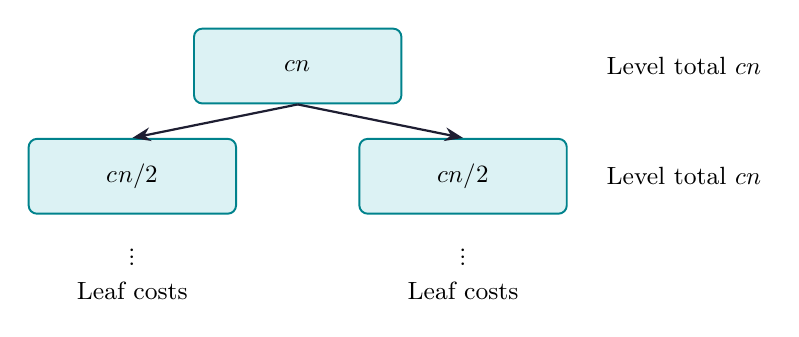
\begin{tikzpicture}[every node/.style={font=\small}]
\node[block] (root) at (0,2.1) {$cn$};
\node[block] (a) at (-2.1,0.7) {$cn/2$};
\node[block] (b) at (2.1,0.7) {$cn/2$};
\draw[arrow] (root.south) -- (a.north);
\draw[arrow] (root.south) -- (b.north);
\node[align=center] at (-2.1,-0.55) {$\vdots$\\[2pt] Leaf costs};
\node[align=center] at (2.1,-0.55) {$\vdots$\\[2pt] Leaf costs};
\node[anchor=west] at (3.8,2.1) {Level total $cn$};
\node[anchor=west] at (3.8,0.7) {Level total $cn$};
\end{tikzpicture}\par
\end{tcolorbox}

\begin{tcolorbox}[examplebox, title={A tree dominated by its leaves}]
For $T(n)=3T(n/2)+n$, level $i$ has $3^i$ subcalls of size $n/2^i$ and costs $n(3/2)^i$. If $h=\log_2 n$, there are $3^h=n^{\log_2 3}$ leaves. The internal level costs form a geometric progression with ratio $3/2$.
\[
n\sum_{i=0}^{h-1}(3/2)^i
  =2n\left((3/2)^h-1\right)
  =\Theta(n^{\log_2 3}).
\]
Including constant-cost leaves leaves the same final order.
\end{tcolorbox}

\subsection{Master theorem and its limits}
\begin{tcolorbox}[formulabox, title={Master theorem for equal subproblem sizes}]
Let $T(n)=aT(n/b)+f(n)$ with $a\ge1$, $b>1$, a constant-size base case and $p=\log_b a$. The following common forms apply.
\begin{enumerate}[leftmargin=*, itemsep=3pt, topsep=4pt]
  \item \textbf{Leaves dominate.} If $f(n)=O(n^{p-\varepsilon})$ for some $\varepsilon>0$, then $T(n)=\Theta(n^p)$.
  \item \textbf{Balanced levels.} If $f(n)=\Theta(n^p\log^k n)$ with $k\ge0$, then $T(n)=\Theta(n^p\log^{k+1}n)$. The basic exam case has $k=0$.
  \item \textbf{Root dominates.} If $f(n)=\Omega(n^{p+\varepsilon})$ and $af(n/b)\le c f(n)$ eventually for some $c<1$, then $T(n)=\Theta(f(n))$.
\end{enumerate}
\end{tcolorbox}

\par\vspace{5pt}
\begingroup
\setlength{\extrarowheight}{1pt}
\noindent\begin{tabularx}{\linewidth}{|B{4.4cm}|Y|Y|}
\hline
\textbf{Recurrence} & \textbf{Check} & \textbf{Answer} \\ \hline
$4T(n/2)+n$ & $p=2$ and $n$ is polynomially smaller than $n^2$. & $\Theta(n^2)$ \\ \hline
$2T(n/2)+n\log n$ & $p=1$, $k=1$. & $\Theta(n\log^2 n)$ \\ \hline
$2T(n/2)+n^2$ & $p=1$ and $2(n/2)^2=n^2/2$. & $\Theta(n^2)$ \\ \hline
\end{tabularx}\par
\endgroup
\begin{tcolorbox}[masonbox, title={When to choose another method}]
A recurrence with calls of sizes $n-1$, $n/3$ and $2n/3$ does not have the required equal-size pattern. For $T(n)=T(n-1)+n$, expanding yields $T(1)+\sum_{j=2}^n j=\Theta(n^2)$. For borderline functions outside the stated Master cases, use a recursion tree or prove an inductive bound directly.
\end{tcolorbox}

\newpage
\begin{center}
  {\large\bfseries\color{myred} Quick Revision --- Module 1}\\[3pt]
  {\small\color{mydark} Algorithm Analysis and Recurrence Relations $|$ ES-CS401}
\end{center}
\noindent{\color{myred}\rule{\linewidth}{1.2pt}}\par\vspace{4pt}

\begin{tcolorbox}[formulabox, title={Key Concepts at a Glance}]
\renewcommand{\arraystretch}{1.35}
\noindent\begin{tabularx}{\linewidth}{B{4.5cm}Y}
Worst-case time & $\max_{I\in\mathcal I_n} C(I)$ over all size-$n$ inputs. \\[3pt]
Average-case time & $\mathbb E[C(I)]$ under the stated input model. \\[3pt]
Triangular loop & $\sum_{i=1}^n i=n(n+1)/2$. \\[3pt]
Divide-and-conquer threshold & Compare $f(n)$ with $n^{\log_b a}$ for $aT(n/b)+f(n)$. \\[3pt]
\end{tabularx}\par
\end{tcolorbox}

\begin{tcolorbox}[defbox, title={One-Line Definitions}]
\begin{itemize}[leftmargin=*, itemsep=3pt, topsep=4pt]
  \item \textbf{Algorithm.} A finite specification of effective steps for a problem.
  \item \textbf{Loop invariant.} A property maintained across iterations.
  \item \textbf{Auxiliary space.} Peak working memory beyond the stated input and output convention.
  \item \textbf{Base case.} A small input solved directly, without further recursion.
\end{itemize}
\end{tcolorbox}

\begin{tcolorbox}[exambox, title={Frequently Asked / Viva Questions}]
\begin{enumerate}[topsep=0pt, label=\textbf{Q\arabic*.}, itemsep=5pt, leftmargin=*]
  \item \Q{What are the five standard characteristics?}
    Input, output, definiteness, finiteness and effectiveness.
  \item \Q{What establishes total correctness?}
    Partial correctness together with termination.
  \item \Q{How is a tight asymptotic bound written?}
    Use $\Theta$ after proving matching upper and lower orders.
  \item \Q{Does Big-O mean worst case?}
    Big-O is an upper bound that can be applied to any specified case function.
  \item \Q{When is linear search fastest?}
    A nonempty array whose first element matches needs one comparison.
  \item \Q{Why does average case need a distribution?}
    Each possible operation count must be weighted by its probability.
  \item \Q{What must an empirical comparison control?}
    Input size, workload family, machine, implementation settings and trial procedure.
  \item \Q{How much stack space does recursive binary search use?}
    $O(\log n)$ frames when calls are not eliminated.
  \item \Q{Why is the recursive base case essential?}
    It anchors both termination and the recurrence solution.
  \item \Q{What does the recursion tree method sum?}
    Non-recursive work at each level plus the cost of the leaves.
  \item \Q{Solve $T(n)=2T(n/2)+n$.}
    Each internal level costs $n$ and there are $\log_2 n$ levels, giving $\Theta(n\log n)$.
  \item \Q{Can the Master theorem solve a decrement-by-one recurrence?}
    Use expansion or substitution because the smaller call does not shrink by a constant factor.
\end{enumerate}
\end{tcolorbox}

\begin{tcolorbox}[tikzbox, title={Summary Comparison}]
\par\vspace{5pt}
\begingroup
\setlength{\extrarowheight}{1pt}
\noindent\begin{tabularx}{\linewidth}{|B{3.45cm}|Y|Y|}
\hline
\textbf{Method} & \textbf{Best used when} & \textbf{Check before finishing} \\ \hline
Substitution & A likely bound is available. & Check constants, base cases and the induction hypothesis. \\ \hline
Recursion tree & Level costs can be counted. & Include leaves and sum the complete series. \\ \hline
Master theorem & Calls split into equal-size subproblems. & Check the correct case and any regularity requirement. \\ \hline
\end{tabularx}\par
\endgroup
\end{tcolorbox}


% -- Module 2 -----------------------------------------------------------------
\modulestart{2}{Algorithm Design Strategies}

\section{Algorithm Design Strategies}
\begin{tcolorbox}[defbox, title={Feasible solutions and objective functions}]
A \textbf{feasible solution} satisfies the problem's constraints. An \textbf{objective function} assigns a cost or value to each feasible solution. An optimisation algorithm seeks the feasible solution of minimum cost or maximum value.
\end{tcolorbox}

\subsection{Brute force and divide and conquer}
\textbf{Brute force} checks every candidate under an explicit enumeration rule. It is easy to justify: the enumeration includes every possible optimum, and the algorithm chooses the best feasible candidate. This is useful for small instances, test oracles and establishing a baseline.
\begin{tcolorbox}[examplebox, title={Counting exhaustive candidates}]
A subset problem on $n$ items has $2^n$ inclusion patterns. If testing each from scratch costs $O(n)$, exhaustive search takes $O(n2^n)$. A travelling salesperson tour fixing the start has $(n-1)!$ visit orders, with half as many distinct tours in the symmetric case for $n\ge3$ when reversal is identified.
\end{tcolorbox}

\textbf{Divide and conquer} solves smaller subproblems and combines their answers. Merge sort independently sorts its two halves and merges them. Dynamic programming reuses previously computed states when distinct recursive paths would repeat the same work.

\subsection{Designing a divide-and-conquer algorithm}
\begin{tcolorbox}[examplebox, title={Merge sort from design to correctness proof}]
\begin{enumerate}[leftmargin=*, itemsep=3pt]
  \item \textbf{Divide.} Stop on zero or one key. Otherwise split the array into two halves.
  \item \textbf{Conquer.} Recursively sort each half. By induction on input length, both recursive results are sorted and contain their original keys.
  \item \textbf{Combine.} Compare the first unused key of each half. Append the smaller key and advance its pointer. When one half runs out, append the other's remainder. Each chosen head is the smallest remaining key, so the output remains sorted. Every key is copied once.
\end{enumerate}
{\interlinepenalty=10000 For example, split $(7,2,5,1)$ into $(7,2)$ and $(5,1)$. After the recursive calls, merge $(2,7)$ and $(1,5)$. Pick $1,2,5$ in order, then append $7$. The halves shrink on each recursive call and each merge consumes a key at every step, so the procedure terminates.\par}
\end{tcolorbox}

For powers of two, the two recursive calls and the linear merge give $T(n)=2T(n/2)+\Theta(n)$. The proof in Module 1 gives $\Theta(n\log n)$ time. An array implementation with one reused merge buffer uses $O(n)$ auxiliary storage, including its logarithmic call stack.

\subsection{Greedy choice and the exchange argument}
\begin{tcolorbox}[defbox, title={Greedy algorithm}]
A \textbf{greedy algorithm} commits to a locally preferred feasible choice according to a rule. To prove exactness, show that some optimum can include that choice, then prove that applying the rule to the remaining instance preserves optimality.
\end{tcolorbox}

\begin{tcolorbox}[examplebox, title={Interval scheduling by earliest finish}]
To schedule the maximum number of non-overlapping intervals, sort by finish time and repeatedly take the first interval whose start is at least the last chosen finish. Suppose an optimal schedule begins with interval $o$ and the greedy algorithm chooses $g$. Then $f(g)\le f(o)$. Replacing $o$ by $g$ preserves feasibility and count, because every later interval starts at or after $f(o)$. Repeat the argument on the remaining intervals. Sorting costs $O(n\log n)$ and the scan costs $O(n)$.
\end{tcolorbox}

A rule can be fast without being optimal. In the $0/1$ knapsack example below, value density supplies a good fractional solution and an upper bound for search, while the exact discrete solution needs a different argument.

\subsection{Dynamic programming and its proof pattern}
\begin{tcolorbox}[defbox, title={Dynamic programming}]
\textbf{Dynamic programming (DP)} computes answers for subproblems represented by states. Optimal substructure allows a state to be solved using smaller states. Overlap makes saving answers useful. A state must store all information that can affect its future choices.
\end{tcolorbox}

\begin{enumerate}[leftmargin=*, itemsep=3pt, topsep=4pt]
  \item \textbf{Define the state in words.} Specify what its indices and answer mean.
  \item \textbf{List the final decisions.} Derive a recurrence by including every possible decision and combining it with the appropriate smaller state.
  \item \textbf{Set the base cases.} Give answers for empty or terminal states and distinguish them from impossible states.
  \item \textbf{Choose the order.} Memoisation computes reachable states on demand. Tabulation schedules states after their dependencies.
  \item \textbf{Prove and reconstruct.} Induct over the order of computation. Keep decisions or retrace valid choices in the table to recover an actual optimum.
\end{enumerate}
\textbf{Complexity rule.} Multiply the number of states by the worst work per state when a uniform upper bound applies. Count table memory separately from reconstruction memory.

\subsection{Backtracking and branch-and-bound}
\begin{tcolorbox}[defbox, title={Backtracking and branch-and-bound}]
\textbf{Backtracking} explores choices and retreats when the current partial assignment cannot lead to a feasible solution. \textbf{Branch-and-bound} additionally uses an optimistic objective bound to discard any subproblem that cannot improve the best complete solution found so far, called the incumbent.
\end{tcolorbox}

\begin{tcolorbox}[tikzbox, title={A state-space tree with two kinds of pruning}]
\centering
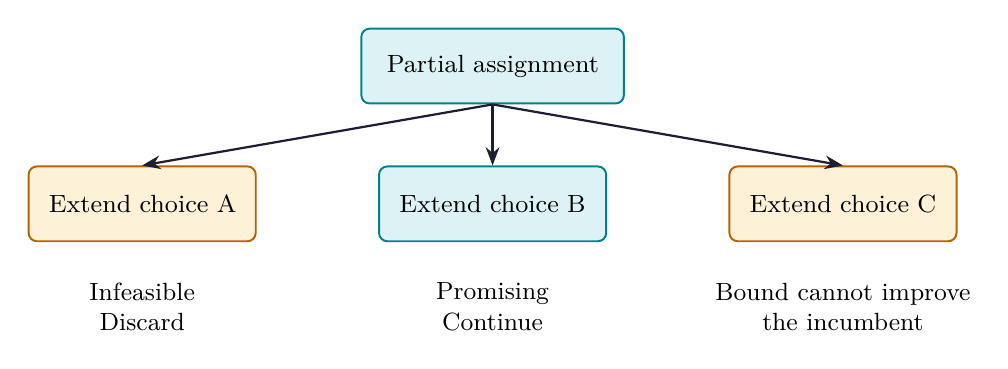
\begin{tikzpicture}[every node/.style={font=\small}]
\node[block,text width=3.1cm] (root) at (0,2.9) {Partial assignment};
\node[amberblock,text width=2.65cm] (left) at (-4.45,1.15) {Extend choice A};
\node[block,text width=2.65cm] (mid) at (0,1.15) {Extend choice B};
\node[amberblock,text width=2.65cm] (right) at (4.45,1.15) {Extend choice C};
\draw[arrow] (root.south) -- (left.north);
\draw[arrow] (root.south) -- (mid.north);
\draw[arrow] (root.south) -- (right.north);
\node[align=center] at (-4.45,-0.16) {Infeasible\\Discard};
\node[align=center] at (0,-0.16) {Promising\\Continue};
\node[align=center] at (4.45,-0.16) {Bound cannot improve\\the incumbent};
\end{tikzpicture}\par
\end{tcolorbox}

\par\vspace{5pt}
\begingroup
\setlength{\extrarowheight}{1pt}
\noindent\begin{tabularx}{\linewidth}{|B{3.55cm}|Y|Y|}
\hline
\textbf{Method} & \textbf{Tests before descending} & \textbf{Typical traversal} \\ \hline
Backtracking & Can this prefix still satisfy every constraint? & Depth-first with a recursion stack. \\ \hline
Branch-and-bound & Can any feasible completion beat the incumbent? & Depth-first, breadth-first or best-bound with a priority queue. \\ \hline
Brute force & Only the completed candidate is checked in the simplest method. & Enumerate the full candidate space. \\ \hline
\end{tabularx}\par
\endgroup
\begin{tcolorbox}[formulabox, title={Safe objective pruning}]
For minimisation, discard a node when its lower bound is at least the incumbent cost. For maximisation, discard it when its upper bound is at most the incumbent value. These comparisons find one optimum. Retain equality if every optimal solution must be listed.
\end{tcolorbox}

\begin{tcolorbox}[examplebox, title={Backtracking for subset sum}]
For nonnegative items $(3,5,6)$ and target $8$, branch on taking or skipping each item. From prefix $(3,5)$ the sum is $8$ and a valid subset is found. The prefix $(3,6)$ has sum $9$ and can be pruned, because further nonnegative items cannot reduce it. A partial sum plus the sum of all remaining items below $8$ also permits pruning. If negatives are allowed, these two bounds require modification.
\end{tcolorbox}

Both searches may still visit exponentially many nodes. A good branching order may find a strong incumbent early, but it does not change the exactness argument.

\section{Bin Packing, Knapsack and Travelling Salesperson}
Bin packing minimises the number of bins, knapsack maximises selected value under a capacity, and TSP minimises the cost of a complete tour.
\subsection{Bin packing and placement heuristics}
\begin{tcolorbox}[defbox, title={One-dimensional bin packing}]
Each item has a positive size at most the bin capacity $C$. Pack all items using the fewest bins, ensuring the total size assigned to each bin is at most $C$. The number of bins is the objective, while item placement is the decision.
\end{tcolorbox}

\begin{itemize}[leftmargin=*, itemsep=3pt, topsep=4pt]
  \item \textbf{Next Fit.} Try only the current bin. Open a new one when the item does not fit.
  \item \textbf{First Fit.} Scan bins in opening order and choose the first with enough space.
  \item \textbf{Best Fit.} Choose the feasible bin with the smallest remaining capacity after placement.
  \item \textbf{First Fit Decreasing (FFD).} Sort all sizes from largest to smallest, then use First Fit. Reordering requires access to the complete input.
\end{itemize}
\begin{tcolorbox}[examplebox, title={Trace and optimality check with capacity 10}]
The input is $(4,4,6,6)$. First Fit places the two $4$s together, then opens a bin for each $6$. FFD processes $(6,6,4,4)$ and pairs each $6$ with a $4$. Since the total size is $20$, the volume lower bound is $\lceil20/10\rceil=2$. FFD attains that bound in this instance.
\end{tcolorbox}

An exact depth-first search tries placing the next item in any bin where it fits, or opening a new one. Equivalent placements in bins with equal free space can be skipped: swapping those bins maps completions one-to-one. For minimisation, a bound is
\[
b+\left\lceil \frac{\max(0,R-F)}{C}\right\rceil,
\]
where $b$ bins are already open, $F$ is their combined free space and $R$ is the total size still unpacked. Even when pieces cannot fill $F$ perfectly, this estimate is safely optimistic.

\subsection{Fractional and zero-one knapsack}
\begin{tcolorbox}[defbox, title={Knapsack variants}]
Select items of weights $w_i>0$ and nonnegative values $v_i$ subject to capacity $W$. Fractional knapsack allows any portion of each item and scales value proportionally. Zero-one knapsack requires taking an item whole or leaving it.
\end{tcolorbox}

\begin{tcolorbox}[examplebox, title={Why density is exact for fractional knapsack}]
Order by $v_i/w_i$. If a solution takes some lower-density weight while higher-density weight is still available, swap equal amounts of those weights. The total weight is unchanged and the value cannot decrease. Repeating the exchange yields a solution with whole items in density order and at most one partially selected final item. Sorting and scanning take $O(n\log n)$ time.
\end{tcolorbox}

For capacity $50$ and items $(w,v)=(10,60),(20,100),(30,120)$, the density order is $6,5,4$. The fractional value is $60+100+(20/30)120=240$. The corresponding whole-item greedy rule takes items 1 and 2 for value $160$. Items 2 and 3 attain $220$, so the greedy rule is not exact for this zero-one instance.
\begin{tcolorbox}[formulabox, title={Zero-one recurrence and complexity}]
For positive integer weights, let $D[i,c]$ be the best value from the first $i$ items with capacity $c$. Start with $D[0,c]=0$. For $i\ge1$,
\[
D[i,c]=
\begin{cases}
D[i-1,c], & c<w_i,\\
\max\{D[i-1,c],v_i+D[i-1,c-w_i]\}, & c\ge w_i .
\end{cases}
\]
Every feasible optimum either excludes or includes the last item, which proves the two alternatives. The $O(nW)$ time bound is pseudo-polynomial because $W$ may be exponential in its binary encoding length. The full table uses $O(nW)$ space.
\end{tcolorbox}

\begin{tcolorbox}[examplebox, title={Fill a small DP and recover the selection}]
Let $(w,v)=(2,3),(3,4),(4,5)$ and $W=5$.
\par\vspace{5pt}
\begingroup
\setlength{\extrarowheight}{1pt}
\noindent\begin{tabularx}{\linewidth}{|B{2.55cm}|Y|Y|Y|Y|Y|Y|}
\hline
\textbf{Capacity} & \textbf{0} & \textbf{1} & \textbf{2} & \textbf{3} & \textbf{4} & \textbf{5} \\ \hline
No items & 0 & 0 & 0 & 0 & 0 & 0 \\ \hline
Item 1 & 0 & 0 & 3 & 3 & 3 & 3 \\ \hline
Items 1--2 & 0 & 0 & 3 & 4 & 4 & 7 \\ \hline
Items 1--3 & 0 & 0 & 3 & 4 & 5 & 7 \\ \hline
\end{tabularx}\par
\endgroup
At $(3,5)$ the value is unchanged from row 2, so item 3 can be skipped. At $(2,5)$, $4+D[1,2]=7$ improves on skipping item 2. The remaining capacity is 2 and item 1 completes the optimum.
\end{tcolorbox}

With one array, process capacities from $W$ down to $w_i$ for each item. Then $D[c-w_i]$ is still from the previous row when $D[c]$ is updated. Ascending iteration can reuse item $i$ within the same round. One-row memory is $O(W)$ for computing the value.
\begin{tcolorbox}[examplebox, title={A fractional upper bound in zero-one branch-and-bound}]
In the capacity-$50$ instance, first obtain a feasible incumbent of value $220$ using items 2 and 3. On the branch that includes item 1 and excludes item 2, at most $40$ capacity remains and only item 3 is available. Its fractional relaxation gives $60+120=180$. Prune the branch. On the branch excluding item 1, the upper bound is $220$. On the branch containing items 1 and 2, item 3 is infeasible as a whole, so its best complete value is $160$. This covers every branch and proves $220$ optimal.
\end{tcolorbox}

\subsection{Travelling salesperson problem and route design}
\begin{tcolorbox}[defbox, title={Travelling salesperson problem (TSP)}]
Given a distance or cost for travelling between cities, find a least-cost tour that starts at one city, visits every other city exactly once, and returns to the start. Distances may be symmetric. A \textbf{metric} TSP additionally obeys the triangle inequality.
\end{tcolorbox}

\begin{itemize}[leftmargin=*, itemsep=3pt, topsep=4pt]
  \item \textbf{Brute force.} Fix the starting city, enumerate permutations and include the return edge in every cost.
  \item \textbf{Backtracking.} Extend the route with an unvisited city. Reject an illegal edge or a move that would repeat a city.
  \item \textbf{Branch-and-bound.} For a symmetric instance and a nonempty unvisited set $U$, add three terms to the prefix cost: an MST on $U$, the cheapest edge from the current endpoint to $U$, and the cheapest edge from $U$ back to the start. Every completion contains such a connection at both ends and a spanning path through $U$. If $U$ is empty, add the actual return edge.
  \item \textbf{Heuristic.} Nearest neighbour chooses the cheapest edge to an unvisited city. A local improvement such as 2-opt replaces two tour edges by reversing a segment when the symmetric tour becomes shorter.
\end{itemize}
\begin{tcolorbox}[formulabox, title={Held--Karp subset DP}]
Fix start $s$ and use $D[S,j]$ for the cheapest path from $s$ visiting exactly the other cities in nonempty $S$, ending at $j\in S$. Then
\begin{align*}
D[\{j\},j]&=c(s,j),\\
D[S,j]&=\min_{i\in S\setminus\{j\}}\{D[S\setminus\{j\},i]+c(i,j)\}.
\end{align*}
The recurrence examines every possible penultimate city. With $U$ equal to all non-start cities, close the tour using $\min_{j\in U}(D[U,j]+c(j,s))$. Time is $O(n^2 2^n)$ and space is $O(n2^n)$. Store the minimising predecessor to recover the tour.
\end{tcolorbox}

\begin{tcolorbox}[examplebox, title={Four-city TSP and a greedy counterexample}]
Let the symmetric edge costs be $AB=10$, $AC=15$, $AD=20$, $BC=35$, $BD=25$ and $CD=30$. From start $A$, the three tours up to reversal cost
\begin{align*}
A\!-\!B\!-\!C\!-\!D\!-\!A &: 10+35+30+20=95,\\
A\!-\!B\!-\!D\!-\!C\!-\!A &: 10+25+30+15=80,\\
A\!-\!C\!-\!B\!-\!D\!-\!A &: 15+35+25+20=95.
\end{align*}
Nearest neighbour from $A$ gives cost $80$. From $D$ it chooses $D,A,B,C,D$ for $95$. The result can depend on the start.
\par
\textbf{Trace one Held--Karp state.} With start $A$, the path to $D$ through $C$ costs $15+30=45$. The path to $C$ through $D$ costs $20+30=50$. To end at $B$ after visiting all three cities, compare the two penultimate cities:
\[
\begin{aligned}
D[\{B,C,D\},B]&=\min\{50+35,\ 45+25\}\\
               &=70.
\end{aligned}
\]
The paths ending at $C$ and $D$ have costs $65$ and $75$. After adding the return edges, the candidates are $80$, $80$ and $95$. The optimal tour has cost $80$.
\end{tcolorbox}

\subsection{Heuristic characteristics and application domains}
\begin{tcolorbox}[defbox, title={Heuristic}]
A \textbf{heuristic} is a practical rule for finding good feasible solutions with limited time or memory. Results can depend on input order, tie-breaking and starting point. An approximation algorithm adds a proved quality guarantee.
\begin{itemize}[leftmargin=*, itemsep=1pt, topsep=2pt]
  \item \textbf{Packing.} Use First Fit for placement. Compare bin count with a lower bound.
  \item \textbf{Routing.} Use nearest neighbour and 2-opt. Compare tour costs across starts.
  \item \textbf{Scheduling.} Rank jobs by urgency. Check lateness and missed deadlines.
\end{itemize}
\end{tcolorbox}

\newpage
\begin{center}
  {\large\bfseries\color{myred} Quick Revision --- Module 2}\\[3pt]
  {\small\color{mydark} Algorithm Design Strategies $|$ ES-CS401}
\end{center}
\noindent{\color{myred}\rule{\linewidth}{1.2pt}}\par\vspace{4pt}

\begin{tcolorbox}[formulabox, title={Key Concepts at a Glance}]
\renewcommand{\arraystretch}{1.35}
\noindent\begin{tabularx}{\linewidth}{B{4.5cm}Y}
Brute force & $2^n$ subsets or $(n-1)!$ fixed-start orders before symmetry reductions. \\[3pt]
Bin packing lower bound & $\lceil\sum_i s_i/C\rceil$ by total volume. \\[3pt]
Knapsack DP & $O(nW)$ time for integer capacity $W$, pseudo-polynomial. \\[3pt]
TSP subset DP & $O(n^2 2^n)$ time and $O(n2^n)$ space. \\[3pt]
Bound directions & Minimisation uses a lower bound on a node. Maximisation uses an upper bound. \\[3pt]
\end{tabularx}\par
\end{tcolorbox}

\begin{tcolorbox}[defbox, title={One-Line Definitions}]
\begin{itemize}[leftmargin=*, itemsep=3pt, topsep=4pt]
  \item \textbf{Greedy choice.} A locally preferred decision committed under a fixed rule.
  \item \textbf{Incumbent.} The best complete feasible solution found so far.
  \item \textbf{State-space tree.} A tree whose branches extend a partial assignment.
  \item \textbf{Heuristic.} A practical search or selection rule whose quality can depend on the instance.
\end{itemize}
\end{tcolorbox}

\begin{tcolorbox}[exambox, title={Frequently Asked / Viva Questions}]
\begin{enumerate}[topsep=0pt, label=\textbf{Q\arabic*.}, itemsep=5pt, leftmargin=*]
  \item \Q{Why is exhaustive search correct?}
    It examines every possible optimum before choosing the best feasible candidate.
  \item \Q{How do exchange arguments work?}
    Replace a choice in an optimum by a greedy one without loss, then repeat on the remaining instance.
  \item \Q{What makes DP useful?}
    Smaller states determine larger ones, and storing repeated states avoids duplicate work.
  \item \Q{How does memoisation differ from tabulation?}
    Memoisation follows recursive dependencies on demand. Tabulation uses an explicit dependency order.
  \item \Q{Why must one-row zero-one DP run backward?}
    It avoids selecting the new item multiple times during the same iteration.
  \item \Q{Why is fractional knapsack useful inside branch-and-bound?}
    It relaxes the restrictions and provides an upper bound on achievable value.
  \item \Q{What does backtracking prune?}
    A prefix that cannot lead to any feasible completion.
  \item \Q{What does branch-and-bound prune?}
    A subtree whose optimistic value cannot improve the incumbent.
  \item \Q{Which packing rule requires the whole input?}
    First Fit Decreasing sorts sizes before placing items.
  \item \Q{What edge is easy to forget in TSP?}
    The return edge from the last visited city to the start.
  \item \Q{What is a safe way to assess a heuristic?}
    Check feasibility, solution value, runtime and comparisons against lower bounds or exact small cases.
\end{enumerate}
\end{tcolorbox}

\begin{tcolorbox}[tikzbox, title={Summary Comparison}]
\par\vspace{5pt}
\begingroup
\setlength{\extrarowheight}{1pt}
\noindent\begin{tabularx}{\linewidth}{|B{3.45cm}|Y|Y|}
\hline
\textbf{Strategy} & \textbf{Main condition or mechanism} & \textbf{Typical use} \\ \hline
Greedy & Safe choices established by an exchange or cut proof. & Interval scheduling and fractional knapsack. \\ \hline
Dynamic programming & A tractable collection of reusable states. & Integer knapsack and subset TSP. \\ \hline
Backtracking & Constraint-based pruning. & Feasible subsets and route enumeration. \\ \hline
Branch-and-bound & Objective-based pruning with an incumbent. & Exact packing, knapsack and TSP. \\ \hline
\end{tabularx}\par
\endgroup
\end{tcolorbox}


% -- Module 3 -----------------------------------------------------------------
\modulestart{3}{Graph and Tree Algorithms}

\section{Graph and Tree Algorithms}
\subsection{Graph representation and basic terminology}
\begin{tcolorbox}[defbox, title={Graph and tree}]
A graph $G=(V,E)$ has vertices and edges. An edge may have a direction, a weight, or both. A tree is a connected acyclic undirected graph. A forest is a collection of trees. Vertices of a rooted tree can be viewed as parents and children starting at a chosen root.
\end{tcolorbox}

\par\vspace{5pt}
\begingroup
\setlength{\extrarowheight}{1pt}
\noindent\begin{tabularx}{\linewidth}{|B{3.5cm}|Y|Y|}
\hline
\textbf{Representation} & \textbf{Space} & \textbf{Typical use} \\ \hline
Adjacency list & $\Theta(V+E)$ & Visit just the neighbours of each vertex. Efficient for sparse graphs. \\ \hline
Adjacency matrix & $\Theta(V^2)$ & Test a specific adjacency in $O(1)$ time. Scanning all neighbours of one vertex costs $\Theta(V)$. \\ \hline
Edge list & $\Theta(E)$ edge records, plus any vertex records. & Scan or sort all edges for algorithms such as Bellman--Ford and Kruskal. \\ \hline
\end{tabularx}\par
\endgroup
Here $V$ and $E$ in complexity expressions denote the numbers of vertices and edges. Weighted matrices need a separate marker for a missing edge so that weight zero can still represent a real edge.

\subsection{Breadth-first search}
\begin{tcolorbox}[defbox, title={Breadth-first search (BFS)}]
BFS explores all vertices at distance $d$ from the source before exploring vertices at distance $d+1$, where distance is the number of edges. A FIFO queue maintains this order.
\end{tcolorbox}

\begin{tcolorbox}[formulabox, title={BFS for unweighted shortest paths}]
\begin{verbatim}
BFS(G, s):
    set every distance to infinity and every parent to NIL
    distance[s] = 0
    enqueue s
    while the queue is not empty:
        u = dequeue()
        for each v in Adj[u]:
            if distance[v] is infinity:
                distance[v] = distance[u] + 1
                parent[v] = u
                enqueue v
    return distance, parent
\end{verbatim}
\end{tcolorbox}

\textbf{Correctness.} The first discovered path of length $d$ is valid by following parents. A shorter path would have a predecessor at an earlier level. BFS would have processed that predecessor and discovered the vertex earlier. Assign distance before enqueuing so each vertex enters the queue once. The full traversal costs $O(V+E)$ with adjacency lists and $O(V^2)$ with a matrix. Parents and the queue use $O(V)$ extra memory.

\subsection{Depth-first search and rooted tree traversals}
\begin{tcolorbox}[defbox, title={Depth-first search (DFS)}]
DFS follows a branch until no undiscovered successor remains, then returns to a previous decision. A recursive call stack or explicit stack represents the active path.
\end{tcolorbox}

\begin{tcolorbox}[formulabox, title={DFS with discovery and finishing times}]
\begin{verbatim}
DFS(G):
    mark all vertices WHITE
    clock = 0
    for each vertex u:
        if u is WHITE:
            Visit(u)

Visit(u):
    mark u GRAY and record discovery time with ++clock
    for each v in Adj[u]:
        if v is WHITE:
            parent[v] = u
            Visit(v)
        else if v is GRAY:
            record a back edge in a directed graph
    mark u BLACK and record finish time with ++clock
\end{verbatim}
\end{tcolorbox}

A DFS tree edge first discovers a vertex. In a directed graph a gray target lies on the active ancestor path, so a back edge proves a cycle. Edges to already finished vertices may be forward (to a descendant) or cross (between completed branches). In an undirected graph ignore the reverse copy of the parent tree edge when testing for cycles. A full DFS costs $O(V+E)$ time and $O(V)$ auxiliary space.
\begin{tcolorbox}[tikzbox, title={Directed graph for the traversal and ordering traces}]
\centering
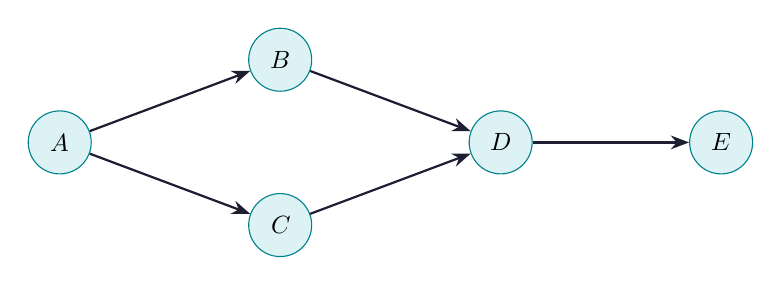
\begin{tikzpicture}[every node/.style={font=\small}]
\tikzset{vertex/.style={circle,draw=myteal,fill=hdrteal,minimum size=8mm,inner sep=0pt}}
\node[vertex] (a) at (0,0) {$A$};
\node[vertex] (b) at (2.8,1.05) {$B$};
\node[vertex] (c) at (2.8,-1.05) {$C$};
\node[vertex] (d) at (5.6,0) {$D$};
\node[vertex] (e) at (8.4,0) {$E$};
\draw[arrow] (a)--(b);
\draw[arrow] (a)--(c);
\draw[arrow] (b)--(d);
\draw[arrow] (c)--(d);
\draw[arrow] (d)--(e);
\end{tikzpicture}\par
\end{tcolorbox}

\begin{tcolorbox}[examplebox, title={BFS levels and DFS times}]
Assume alphabetical neighbour order and source $A$. BFS removes $A,B,C,D,E$ from its queue and records distances $0,1,1,2,3$. The parent of $D$ is $B$, since $B$ is processed before $C$. DFS visits $A,B,D,E$ first. After finishing that branch it visits $C$. The discovery/finish pairs are:
\[
A:(1,10),\quad B:(2,7),\quad C:(8,9),\quad D:(3,6),\quad E:(4,5).
\]
The edge $C\to D$ reaches a completed branch in this DFS.
\end{tcolorbox}

\par\vspace{5pt}
\begingroup
\setlength{\extrarowheight}{1pt}
\noindent\begin{tabularx}{\linewidth}{|B{3.4cm}|Y|Y|}
\hline
\textbf{Rooted tree visit} & \textbf{Order} & \textbf{Typical application} \\ \hline
Preorder & Root, then subtrees. & Copy a hierarchy or emit a prefix expression. \\ \hline
Inorder & Left subtree, root, right subtree in a binary tree. & Read a binary search tree in key order. \\ \hline
Postorder & Subtrees, then root. & Evaluate an expression tree or delete children before the parent. \\ \hline
Level order & Queue from the root, one layer at a time. & List nodes by depth. \\ \hline
\end{tabularx}\par
\endgroup

\section{Shortest Paths and Transitive Closure}
\subsection{Relaxation and Dijkstra's algorithm}
\begin{tcolorbox}[defbox, title={Shortest path and relaxation}]
A shortest path minimises the sum of edge weights between specified vertices. Relaxing an edge $u\to v$ replaces $d[v]$ by $d[u]+w(u,v)$ when that value is smaller, and records $u$ as the predecessor. An infinite label represents no path yet discovered.
\end{tcolorbox}

\begin{tcolorbox}[formulabox, title={Dijkstra with a min-priority queue}]
\begin{verbatim}
Dijkstra(G, s):
    initialise d[s] = 0 and all other distances to infinity
    keep unsettled vertices in a min-priority queue by d
    while the queue is not empty:
        u = extract-min()
        if d[u] is infinity: break
        for each edge u -> v with v unsettled:
            if d[u] + weight(u, v) < d[v]:
                update d[v] and parent[v]
                decrease the queue key of v
    return d, parent
\end{verbatim}
\end{tcolorbox}

\textbf{Why the extracted distance is final.} On any hypothetical shorter path to the extracted vertex, consider the first unsettled vertex. Its settled predecessor would already have relaxed the edge into it. With nonnegative edge weights, the prefix up to that first unsettled vertex costs no more than the shorter path. Its queue key would therefore be smaller than the extracted key, a contradiction.
\begin{tcolorbox}[examplebox, title={Dijkstra trace}]
Use the directed weighted edges $A\to B:4$, $A\to C:1$, $C\to B:2$, $C\to D:5$ and $B\to D:1$. Starting at $A$, settle in this order:
\par\vspace{5pt}
\begingroup
\setlength{\extrarowheight}{1pt}
\noindent\begin{tabularx}{\linewidth}{|B{2.4cm}|Y|Y|Y|}
\hline
\textbf{Settled vertex} & \textbf{$d[B]$} & \textbf{$d[C]$} & \textbf{$d[D]$} \\ \hline
$A$ & $4$ & $1$ & $\infty$ \\ \hline
$C$ & $3$ & $1$ & $6$ \\ \hline
$B$ & $3$ & $1$ & $4$ \\ \hline
$D$ & $3$ & $1$ & $4$ \\ \hline
\end{tabularx}\par
\endgroup
Predecessors recover $A\to C\to B\to D$ of cost $4$. A binary heap gives $O((V+E)\log V)$ time. An array-based minimum scan gives $O(V^2)$ when using an adjacency matrix.
\end{tcolorbox}

\begin{tcolorbox}[masonbox, title={Dijkstra requires nonnegative weights}]
Take $s\to u:2$, $s\to v:5$, $v\to u:-4$. Finalising $u$ at value $2$ misses the better route of cost $1$. The graph does not need a negative cycle for Dijkstra to fail.
\end{tcolorbox}

\subsection{Bellman--Ford and negative cycles}
\begin{enumerate}[leftmargin=*, itemsep=3pt, topsep=4pt]
  \item Set $d[s]=0$ and every other value to infinity.
  \item Repeat up to $V-1$ full passes over all edges, relaxing from finite labels. Stop early if a pass makes no change.
  \item Scan all edges once more. A further improvement from a finite label signals a reachable negative-weight cycle. Such a cycle makes finite minimum walk costs undefined for vertices reachable from it.
\end{enumerate}
\textbf{Proof outline.} Any finite label is the length of a concrete walk. After $k$ complete passes, each walk using at most $k$ edges has had a chance to improve its final label. When no reachable negative cycle is relevant, a shortest path can be chosen simple and uses at most $V-1$ edges. If a reachable negative cycle exists and every edge on it satisfies the no-improvement inequalities, summing those inequalities around the cycle contradicts its negative total weight. Worst-case time is $O(VE)$ for edge scans plus $O(V)$ initialisation.
\begin{tcolorbox}[examplebox, title={A negative edge that Bellman--Ford handles}]
Take $s\to A:4$, $s\to B:5$, $A\to B:-2$, $B\to C:3$, $A\to C:4$. In that edge order, the first pass sets $A=4$, improves $B$ from $5$ to $2$, and sets $C=5$. The result stays unchanged in the next pass. The shortest route to $C$ is $s,A,B,C$, using the negative edge once.
\end{tcolorbox}

For a DAG, process vertices in topological order and relax outgoing edges once. This takes $O(V+E)$ time and supports negative weights because cycles are absent.

\subsection{Floyd--Warshall and Warshall}
\begin{tcolorbox}[defbox, title={Transitive closure}]
The transitive closure records which ordered pairs have a directed path. In a \textbf{reflexive} closure, also include paths of length zero, so every diagonal entry is true.
\end{tcolorbox}

\begin{tcolorbox}[formulabox, title={Two forms of the intermediate-vertex recurrence}]
Order the vertices $1,\dots,V$. At stage $k$ determine whether the best route from $i$ to $j$ can use vertex $k$ in addition to earlier intermediate vertices.
\begin{align*}
D^{(k)}_{ij}
 &=\min\{D^{(k-1)}_{ij},D^{(k-1)}_{ik}+D^{(k-1)}_{kj}\},\\
R^{(k)}_{ij}
 &=R^{(k-1)}_{ij}\lor
   (R^{(k-1)}_{ik}\land R^{(k-1)}_{kj}).
\end{align*}
Use Floyd--Warshall for distance and Warshall for Boolean reachability. Start distances with edge weights, zero on the diagonal in the absence of negative self-loops, and infinity for missing edges. If self-loops are present, initialise each diagonal to the minimum of zero and its loop weight. Start Boolean entries with adjacency and choose the diagonal convention. In either algorithm $k$ is the outer loop. Time is $O(V^3)$ and in-place memory for the matrix is $O(V^2)$.
\end{tcolorbox}

\begin{tcolorbox}[examplebox, title={Intermediate vertex update}]
If $A\to B$ has cost $4$, $B\to C$ cost $2$ and $A\to C$ cost $9$, the stage allowing $B$ improves $D[A,C]$ to $6$. In a Boolean graph with just $A\to B$ and $B\to C$, that same stage sets $R[A,C]$ to true despite no direct edge. A negative diagonal after Floyd--Warshall indicates a negative cycle.
\end{tcolorbox}

\section{Spanning Trees and Topological Ordering}
A minimum spanning tree minimises wiring cost when edges are weighted. A topological order handles a different task: scheduling directed dependencies.
\subsection{Minimum spanning tree and the cut property}
\begin{tcolorbox}[defbox, title={Minimum spanning tree}]
An MST is a spanning tree of minimum total edge weight in a connected undirected weighted graph. It has $V-1$ edges and connects every vertex. A disconnected graph has a minimum spanning forest. The objective is total wiring cost, while a shortest-path tree minimises distances from one source.
\end{tcolorbox}

\textbf{Exchange proof for a safe edge.} A cut partitions the vertices into two sets. Assume the current chosen edges belong to some MST and none crosses this cut. Let $e$ be a minimum-weight crossing edge. If an MST containing the chosen edges omits $e$, adding $e$ forms a cycle containing another crossing edge $f$. Remove $f$. It was not among the chosen edges. Since $w(e)\le w(f)$, the result is also an MST and includes $e$.
\par\vspace{5pt}
\begingroup
\setlength{\extrarowheight}{1pt}
\noindent\begin{tabularx}{\linewidth}{|B{3.0cm}|Y|Y|}
\hline
\textbf{Algorithm} & \textbf{Greedy rule} & \textbf{Cost with common structures} \\ \hline
Kruskal & Sort edges by weight. Accept an edge only when its endpoints belong to different components. & $O(E\log E)$ plus near-linear disjoint-set operations. \\ \hline
Prim & Grow one tree from a start. Add a cheapest edge from the current tree to an outside vertex. & $O((V+E)\log V)$ with a binary heap and adjacency lists. \\ \hline
\end{tabularx}\par
\endgroup
\textbf{Implementation.} In Kruskal, start with one disjoint set per vertex. For each edge in increasing weight order, compare its two set representatives. If they differ, choose the edge and union the sets. In Prim, store each outside vertex's cheapest edge into the current tree. Extract the vertex with minimum key, add its stored edge, and update the keys of its outside neighbours.

\begin{tcolorbox}[examplebox, title={Kruskal and Prim on the same network}]
Let $AB=1$, $BC=2$, $AC=3$, $CD=4$, $BD=5$, $AD=7$. Kruskal accepts $AB$ and $BC$, rejects $AC$ because $A$ and $C$ are already connected, and accepts $CD$. Prim from $D$ takes $DC$ (4), $CB$ (2), then $BA$ (1). Both have cost $7$. Equal-weight edges can give several valid MSTs. Negative edge weights are permitted.
\end{tcolorbox}

\subsection{Topological sorting of a DAG}
\begin{tcolorbox}[defbox, title={Topological order}]
A topological ordering of a directed graph lists every vertex so that each edge $u\to v$ places $u$ before $v$. Such an order exists exactly for a directed acyclic graph (DAG).
\end{tcolorbox}

\begin{tcolorbox}[formulabox, title={Kahn's indegree algorithm}]
\begin{verbatim}
Compute indegree of every vertex.
Enqueue every vertex whose indegree is zero.
While the queue is nonempty:
    remove u and append it to the order
    for each edge u -> v:
        decrement indegree[v]
        if indegree[v] becomes zero:
            enqueue v
If the order has fewer than V vertices, report a cycle.
\end{verbatim}
\end{tcolorbox}

Every removed vertex has no remaining incoming edge. If no vertex can be removed while vertices remain, repeatedly following incoming edges in that finite remainder reaches a cycle. DFS offers another method: reject back edges and output vertices in decreasing finish time. In the traversal example the DFS order is $A,C,B,D,E$. Both methods run in $O(V+E)$ time. Tasks with no dependency between them may appear in either order.

\section{Network Flow Algorithms}
\subsection{Flow, cuts and the residual graph}
\begin{tcolorbox}[defbox, title={Feasible flow}]
A directed network gives each edge a capacity $c(u,v)\ge0$, with source $s$ and sink $t$. A feasible flow satisfies $0\le f(u,v)\le c(u,v)$ and conserves flow at intermediate vertices. The value $|f|$ is the net flow leaving $s$. An $s$--$t$ cut partitions vertices into $S$ and its complement. The cut capacity sums only original edges from $S$ to the complement.
\end{tcolorbox}

The residual graph contains unused forward capacity and reverse arcs that allow a previous allocation to be reduced. For a single original edge, the forward residual is $c-f$ and the reverse residual is $f$. When both directions were originally present, keep their edge contributions distinct or combine them consistently.
\begin{tcolorbox}[formulabox, title={Ford--Fulkerson and Edmonds--Karp}]
\begin{verbatim}
Start with zero flow.
While the residual graph has a path from s to t:
    find the minimum residual capacity on the path
    augment by this bottleneck amount
    update forward and reverse residual capacities
Return the final flow.
For Edmonds--Karp, find each residual path with BFS.
\end{verbatim}
\end{tcolorbox}

\textbf{Max-flow min-cut argument.} Conservation implies that every flow's value is at most any cut capacity. If no augmenting path remains, let $S$ be the residually reachable set from $s$. Every original arc from $S$ to the other side is saturated and any original arc in the reverse direction carries zero. Hence the flow equals the capacity of this cut and is maximum.
\begin{tcolorbox}[tikzbox, title={Flow network for the augmenting-path trace}]
\centering
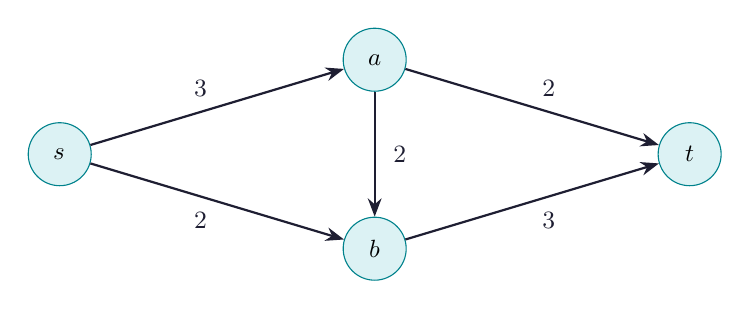
\begin{tikzpicture}[every node/.style={font=\small}]
\tikzset{vertex/.style={circle,draw=myteal,fill=hdrteal,minimum size=8mm,inner sep=0pt}}
\node[vertex] (s) at (0,0) {$s$};
\node[vertex] (a) at (4,1.2) {$a$};
\node[vertex] (b) at (4,-1.2) {$b$};
\node[vertex] (t) at (8,0) {$t$};
\draw[arrow] (s)--node[above left] {3} (a);
\draw[arrow] (s)--node[below left] {2} (b);
\draw[arrow] (a)--node[right=3pt] {2} (b);
\draw[arrow] (a)--node[above right] {2} (t);
\draw[arrow] (b)--node[below right] {3} (t);
\end{tikzpicture}\par
\end{tcolorbox}

\begin{tcolorbox}[examplebox, title={Augmenting paths with cancellation}]
\par\vspace{5pt}
\begingroup
\setlength{\extrarowheight}{1pt}
\noindent\begin{tabularx}{\linewidth}{|B{3.45cm}|Y|Y|}
\hline
\textbf{Residual path} & \textbf{Bottleneck} & \textbf{Flow value afterwards} \\ \hline
$s,a,b,t$ & 2 & 2 \\ \hline
$s,a,t$ & 1 & 3 \\ \hline
$s,b,t$ & 1 & 4 \\ \hline
$s,b,a,t$ & 1 & 5 \\ \hline
\end{tabularx}\par
\endgroup
The last path uses the residual reverse arc $b\to a$, reducing the original flow on $a\to b$ from 2 to 1. The cut $S=\{s\}$ has capacity $3+2=5$. The exhibited feasible flow reaches this upper bound.
\end{tcolorbox}

With integral capacities, Ford--Fulkerson has at most $|f^*|$ augmentations from zero because each increases the value by at least one. With $O(V+E)$ residual searches the total is $O((V+E)|f^*|)$ plus initialisation. This bound depends on capacity magnitude. Edmonds--Karp uses shortest residual paths in number of edges and has the polynomial bound $O(VE^2)$ after isolated vertices are discarded. Uses include matching, bandwidth allocation and project selection.

\subsection{Application: matching as unit-capacity network flow}
A \textbf{matching} is a set of edges sharing no endpoints. To match workers on the left to compatible jobs on the right, add edges of capacity 1 from the source to each worker, from workers to compatible jobs, and from each job to the sink.
\begin{itemize}[leftmargin=*, itemsep=3pt]
  \item A matching of size $k$ creates a flow of value $k$ by sending one unit along each selected worker--job path.
  \item Integral flow cannot use a worker or a job twice because its edge to the source or sink has capacity 1. Read edges carrying one unit to obtain the matching.
  \item Starting from zero and augmenting integral capacities preserves integrality. Max flow therefore returns a maximum-cardinality matching.
\end{itemize}
\begin{tcolorbox}[examplebox, title={Why rerouting beats an early assignment}]
Worker $A$ can do jobs $X$ and $Y$. Worker $B$ can do only $X$. If the first augmenting path assigns $A$ to $X$, use the next residual path $s\to B\to X\to A\to Y\to t$. The reverse arc $X\to A$ cancels $A$'s old assignment. The new matching uses $B$--$X$ and $A$--$Y$. The two source arcs give capacity 2, so the matching is maximum.
\end{tcolorbox}

\newpage
\begin{center}
  {\large\bfseries\color{myred} Quick Revision --- Module 3}\\[3pt]
  {\small\color{mydark} Graph and Tree Algorithms $|$ ES-CS401}
\end{center}
\noindent{\color{myred}\rule{\linewidth}{1.2pt}}\par\vspace{4pt}

\begin{tcolorbox}[formulabox, title={Key Concepts at a Glance}]
\renewcommand{\arraystretch}{1.35}
\noindent\begin{tabularx}{\linewidth}{B{4.5cm}Y}
BFS and DFS & $O(V+E)$ with adjacency lists, $O(V)$ auxiliary memory. \\[3pt]
Shortest paths & Dijkstra for nonnegative edges. Bellman--Ford for negative edges. DAGs permit one topological pass. \\[3pt]
All-pairs and closure & Floyd--Warshall (min plus) and Warshall (Boolean), both $O(V^3)$. \\[3pt]
Residual capacity & Unused forward capacity and reversible past flow. \\[3pt]
Optimal flow certificate & A feasible flow and cut with matching value and capacity. \\[3pt]
\end{tabularx}\par
\end{tcolorbox}

\begin{tcolorbox}[defbox, title={One-Line Definitions}]
\begin{itemize}[leftmargin=*, itemsep=3pt, topsep=4pt]
  \item \textbf{Tree.} A connected undirected graph with no cycle.
  \item \textbf{Relaxation.} Improve the known distance by trying one additional edge.
  \item \textbf{Cut.} A partition of the vertices into two sets.
  \item \textbf{Augmenting path.} A source-to-sink path using positive residual capacities.
\end{itemize}
\end{tcolorbox}

\begin{tcolorbox}[exambox, title={Frequently Asked / Viva Questions}]
\begin{enumerate}[topsep=0pt, label=\textbf{Q\arabic*.}, itemsep=5pt, leftmargin=*]
  \item \Q{Why does BFS use FIFO?}
    The queue processes all vertices of one distance before the next layer.
  \item \Q{Which DFS edge certifies a directed cycle?}
    An edge to a gray ancestor on the active path.
  \item \Q{How is a path reconstructed?}
    Follow predecessors from target to source and reverse the resulting list.
  \item \Q{What breaks Dijkstra?}
    A negative edge can later improve a previously settled label.
  \item \Q{When can Bellman--Ford report a negative cycle?}
    A finite-label relaxation is still possible after the usual passes.
  \item \Q{What is the outer loop in Warshall?}
    The intermediate vertex index.
  \item \Q{Which structure supports Kruskal?}
    Disjoint-set union detects whether endpoints already share a component.
  \item \Q{How many edges are in a spanning tree?}
    $V-1$ for a connected graph with $V$ vertices.
  \item \Q{What happens if Kahn's queue empties early?}
    The remaining directed graph contains a cycle.
  \item \Q{Why include residual reverse arcs?}
    They permit cancellation and rerouting of earlier flow choices.
  \item \Q{How does Edmonds--Karp select paths?}
    It uses BFS to select a path with the fewest residual edges.
\end{enumerate}
\end{tcolorbox}

\begin{tcolorbox}[tikzbox, title={Summary Comparison}]
\par\vspace{5pt}
\begingroup
\setlength{\extrarowheight}{1pt}
\noindent\begin{tabularx}{\linewidth}{|B{3.45cm}|Y|Y|}
\hline
\textbf{Task} & \textbf{Algorithm} & \textbf{Key condition} \\ \hline
Minimum edge count & BFS & Unweighted or uniform unit edge cost. \\ \hline
Minimum total wiring & Prim or Kruskal & Undirected weighted graph. \\ \hline
Prerequisite ordering & Kahn or DFS & Directed acyclic graph. \\ \hline
Maximum throughput & Edmonds--Karp & Nonnegative capacities with a source and sink. \\ \hline
\end{tabularx}\par
\endgroup
\end{tcolorbox}


% -- Module 4 -----------------------------------------------------------------
\modulestart{4}{Computability and NP-Completeness}

\section{Computability and NP-Completeness}
\subsection{Decision problems, computability and tractability}
\begin{tcolorbox}[defbox, title={Decision problem and decider}]
A \textbf{decision problem} asks a yes-or-no question. Its language is the set of encodings whose answer is yes. A \textbf{decider} halts on every input and gives the correct answer. A recogniser must accept yes instances, but may run forever on a no instance.
\end{tcolorbox}

\begin{itemize}[leftmargin=*, itemsep=3pt, topsep=4pt]
  \item \textbf{Search.} Produce a witness, such as a tour of cost at most $B$, if one exists.
  \item \textbf{Optimisation.} Find a solution of minimum cost or maximum value, such as the least-cost tour.
  \item \textbf{Decision.} Ask whether a solution meeting the bound $B$ exists. Define the certificate and its input encoding before assigning a complexity class.
  \item \textbf{Tractable.} In the usual complexity-theory convention, a decision problem is tractable if it can be solved in polynomial time. Constants and polynomial degree still matter in practice. A problem shown NP-hard is usually treated as computationally intractable unless $\mathrm{P}=\mathrm{NP}$.
\end{itemize}
TSP is decidable: exhaustive enumeration terminates even when it takes too much time for large instances. Undecidability is a different limitation. It rules out a decider altogether.
\begin{tcolorbox}[examplebox, title={Why the halting problem is undecidable}]
Suppose a program $H(P,x)$ always decides whether program $P$ halts on input $x$. Construct $D(P)$ that runs forever if $H(P,P)$ says yes, and halts if $H(P,P)$ says no. Run $D$ on its own encoding. If $H(D,D)$ says yes, $D(D)$ runs forever. If it says no, $D(D)$ halts. Either answer contradicts the specification, so no such $H$ exists.
\end{tcolorbox}

\subsection{Polynomial time and polynomial verification}
\begin{tcolorbox}[defbox, title={The classes P and NP}]
$\mathrm{P}$ contains decision problems solvable by a deterministic algorithm in polynomial time. $\mathrm{NP}$ contains decision problems for which every yes instance has a polynomial-length certificate that a deterministic polynomial-time verifier accepts. For a no instance, every proposed certificate must be rejected.
\end{tcolorbox}

\begin{tcolorbox}[formulabox, title={Formal verifier definition}]
A language $L$ is in $\mathrm{NP}$ if a polynomial $p$ and a polynomial-time verifier $V$ exist such that
\[
x\in L \iff \exists\, y,\quad |y|\le p(|x|)\ \text{and}\ V(x,y)=1.
\]
Equivalently, a nondeterministic machine can guess a certificate and verify it on an accepting computation branch within polynomial time.
\end{tcolorbox}

\begin{tcolorbox}[examplebox, title={Verifying the decision version of TSP}]
Given a proposed sequence of cities, check that it lists each city once, that the return edge is valid, and that the sum of weights does not exceed $B$. The certificate has polynomial length. The verifier uses polynomial time including the cost of arithmetic on the encoded weights.
\end{tcolorbox}

Every problem in $\mathrm{P}$ is in $\mathrm{NP}$ because a verifier can simply solve the decision problem. Whether $\mathrm{P}=\mathrm{NP}$ is open. The letters NP refer to nondeterministic polynomial time.

\section{Reductions and Completeness}
\subsection{Polynomial-time many-one reductions}
\begin{tcolorbox}[defbox, title={Polynomial-time reduction}]
For decision problems $A$ and $B$, write $A\le_p B$ when a polynomial-time function $f$ maps each instance of $A$ to an instance of $B$ with $x\in A$ exactly when $f(x)\in B$. Both yes and no answers must be preserved.
\end{tcolorbox}

\begin{tcolorbox}[tikzbox, title={Direction of a polynomial-time reduction}]
\centering
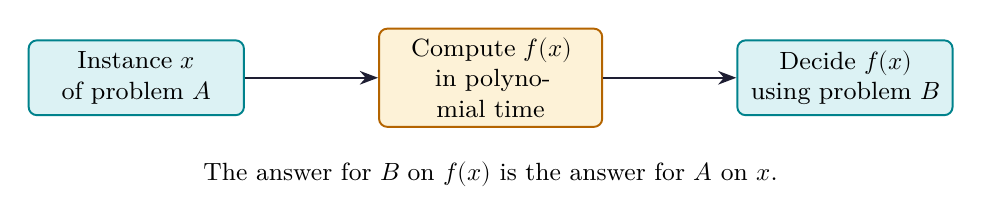
\begin{tikzpicture}[every node/.style={font=\small}]
\node[block,text width=2.5cm] (in) at (0,0) {Instance $x$\\of problem $A$};
\node[amberblock,text width=2.6cm] (f) at (4.5,0) {Compute $f(x)$\\in polynomial time};
\node[block,text width=2.5cm] (out) at (9,0) {Decide $f(x)$\\using problem $B$};
\draw[arrow] (in)--(f);
\draw[arrow] (f)--(out);
\node at (4.5,-1.22) {The answer for $B$ on $f(x)$ is the answer for $A$ on $x$.};
\end{tikzpicture}\par
\end{tcolorbox}

If $A\le_p B$ and $B\in\mathrm P$, then $A\in\mathrm P$: compute the transformation and run the solver for $B$. The output length of the transformation is polynomial because its runtime is polynomial. Composing two such transformations yields a polynomial-time reduction.
\begin{tcolorbox}[defbox, title={NP-hard and NP-complete}]
A problem $B$ is \textbf{NP-hard} if every problem in $\mathrm{NP}$ reduces to it in polynomial time. A decision problem is \textbf{NP-complete} if it is both NP-hard and in $\mathrm{NP}$. NP-hardness on its own supplies no certificate bound. Optimisation problems are commonly called NP-hard when solving them also solves an NP-hard decision version.
\end{tcolorbox}

\begin{enumerate}[leftmargin=*, itemsep=3pt, topsep=4pt]
  \item \textbf{Membership.} Identify a polynomial-length certificate for the target $B$ and give a polynomial-time verifier.
  \item \textbf{Known hardness.} Select an already NP-complete decision problem $A$ with a structure that maps naturally to $B$.
  \item \textbf{Construction.} Map each input $x$ of $A$ to $f(x)$ of $B$. Show that both building time and encoded output size are polynomial.
  \item \textbf{Equivalence.} Prove $x\in A\Rightarrow f(x)\in B$ and the reverse implication separately.
  \item \textbf{Conclusion.} Use transitivity to conclude that $B$ is NP-hard, then add membership to obtain NP-completeness.
\end{enumerate}
\begin{tcolorbox}[masonbox, title={Check the reduction direction}]
Reducing the target to a known NP-complete problem gives an upper bound in terms of that problem. To prove the target hard, reduce the known hard problem \emph{to the target}.
\end{tcolorbox}

\subsection{Cook's theorem: SAT is NP-complete}
\begin{tcolorbox}[defbox, title={SAT, CNF-SAT and 3-SAT}]
SAT asks if some assignment makes a Boolean formula true. CNF-SAT restricts the formula to an AND of clauses, each of which is an OR of literals. A literal is a variable or its negation. In 3-SAT each clause has at most three literals. The conventional exactly-three version can be obtained by padding shorter clauses.
\end{tcolorbox}

\textbf{Cook--Levin theorem.} SAT is NP-complete in the modern polynomial many-one formulation. To show membership in NP, use a truth assignment as the certificate and evaluate the formula. For NP-hardness, let a nondeterministic machine decide some $L\in\mathrm{NP}$ in time $T=p(n)$ on input $x$.
\begin{enumerate}[leftmargin=*, itemsep=3pt, topsep=4pt]
  \item \textbf{Represent the history.} Any accepting run fits in $T+1$ time rows and $O(T)$ tape positions, with one encoded tape symbol per cell and state/head information. The finite machine alphabet and state set are fixed.
  \item \textbf{Initial configuration.} Add clauses requiring the first row to encode the input, initial state, head position and blank remainder.
  \item \textbf{Legal transitions.} Use constraints between successive rows for the machine's step rule. Each step uses one consistent legal nondeterministic choice, updates the head neighbourhood and leaves untouched cells unchanged.
  \item \textbf{Acceptance.} Require an accepting configuration within the time bound. An accepting run can be padded by giving its accepting state an idle self-loop.
  \item \textbf{Equivalence and size.} A legal accepting run satisfies the clauses. A satisfying assignment decodes to a legal accepting run. The tableau and its transition constraints have polynomial size, so the construction is a polynomial-time reduction.
\end{enumerate}
\begin{tcolorbox}[examplebox, title={Splitting a long CNF clause}]
Use a fresh variable $z$ to replace $(a\lor b\lor c\lor d)$ by
\[
(a\lor b\lor z)\land(\neg z\lor c\lor d).
\]
If $a\lor b$ is true, choose $z$ false. If only $c\lor d$ is true, choose $z$ true. If all original literals are false, the two clauses demand both $z$ and $\neg z$. A chain of fresh variables splits longer clauses in linear size, preserving satisfiability.
\end{tcolorbox}

\textbf{Reading.} Stephen A. Cook, \href{https://www.cs.cmu.edu/~15455/resources/Cook1971-complx-thm-proof.pdf}{The Complexity of Theorem-Proving Procedures (1971)}. The paper uses oracle reducibility in its original formulation. The tableau argument above is presented in the modern SAT formulation used in exams.

\section{Standard NP-Complete Problems and Reductions}
\subsection{Decision formulations and certificates}
\par\vspace{5pt}
\begingroup
\setlength{\extrarowheight}{1pt}
\noindent\begin{tabularx}{\linewidth}{|B{3.4cm}|Y|Y|}
\hline
\textbf{Problem} & \textbf{Decision question} & \textbf{Certificate to verify} \\ \hline
3-SAT & Does this 3-CNF formula have a satisfying assignment? & Boolean values for the variables. \\ \hline
Clique & Is there a pairwise adjacent set of at least $k$ vertices? & A set of $k$ vertices and all their pair adjacencies. \\ \hline
Independent Set & Is there a set of at least $k$ pairwise non-adjacent vertices? & A set of $k$ vertices. No selected pair may share an edge. \\ \hline
Vertex Cover & Is there a set of at most $k$ vertices touching every edge? & A set of selected vertices. Check every edge endpoint pair. \\ \hline
Hamiltonian Cycle & Does a graph contain a cycle visiting every vertex once? & The cyclic vertex order and all required edges. \\ \hline
Decision TSP & Is some tour's total weight at most $B$? & A tour and its verified total cost. \\ \hline
Subset Sum & Can some subset of the input integers sum exactly to $B$? & An inclusion bit for each input item. \\ \hline
Decision Knapsack & Can selected items fit weight $W$ and attain value at least $K$? & An inclusion bit for each item. Verify both totals. \\ \hline
\end{tabularx}\par
\endgroup
The cited decision problems are standard NP-complete versions with their usual unrestricted inputs. Restricted cases may have faster algorithms. For example, Hamiltonian cycle is about visiting vertices once, whereas Eulerian cycle uses each edge once and has a polynomial-time test.

\subsection{Reduction from 3-SAT to Clique}
\begin{tcolorbox}[examplebox, title={Literal-occurrence graph}]
Let the 3-CNF input have $m$ clauses.
\begin{enumerate}[leftmargin=*, itemsep=3pt, topsep=4pt]
  \item Make one vertex per literal occurrence and mark its clause. Put no edge within a clause.
  \item Between different clauses, put an edge when the two literals are compatible, meaning neither is the negation of the other.
  \item Ask whether the graph has a clique of size $m$. There are at most $3m$ vertices and $O(m^2)$ edges.
\end{enumerate}
\textbf{Forward direction.} A satisfying assignment makes some literal true in each clause. Choose one true occurrence from each. True literals cannot contradict each other, so the chosen vertices form a clique.
\par
\textbf{Reverse direction.} An $m$-clique contains at most one vertex per clause, so it contains one from each. Its literals are pairwise compatible. Assign them true and choose the remaining variables arbitrarily. Each clause is satisfied.
\par
For $(x\lor y\lor\neg z)\land(\neg x\lor z\lor y)\land(x\lor\neg y\lor z)$, choose occurrences $x$, $y$ and $x$ from the three clauses. The occurrence of $x$ in each clause is a separate vertex. Setting $x$ and $y$ true satisfies the formula.
\end{tcolorbox}

\subsection{Graph complements and the cover relationship}
A set $S$ is a clique in $G$ exactly when it is independent in the complement $\overline G$. Also, $S$ is independent in a graph $H$ exactly when $V(H)\setminus S$ covers all edges. The latter equivalence holds because an uncovered edge would have both endpoints in $S$. Thus
\[
(G,k)_{\mathrm{Clique}}\mapsto
(\overline G,|V|-k)_{\mathrm{Vertex\ Cover}}
\]
preserves answers and is polynomial to construct.

\subsection{Hamiltonian Cycle to TSP and Subset Sum to Knapsack}
\begin{tcolorbox}[examplebox, title={TSP with costs 1 and 2}]
For an undirected graph on $n\ge3$ vertices, make a complete weighted graph on the same vertices. Use cost $1$ for original edges and $2$ for nonedges. Set the decision budget to $n$. A Hamiltonian cycle in the original graph gives $n$ cost-$1$ edges. Conversely every tour uses exactly $n$ edges of cost at least $1$. It can reach the budget only by using original edges throughout. This construction also satisfies the triangle inequality.
\end{tcolorbox}

\begin{tcolorbox}[examplebox, title={Decision Knapsack from Subset Sum}]
Given positive integers $a_i$ and target $B$, define item $i$ to have $w_i=v_i=a_i$ and choose $W=K=B$. A subset summing to $B$ is feasible and attains the value threshold. A feasible selection reaching the threshold has the same weight and value, so its sum is forced to equal $B$. The transformation copies only polynomially many bits.
\end{tcolorbox}

\begin{tcolorbox}[masonbox, title={What completeness lets you conclude}]
A polynomial-time algorithm for one NP-complete problem would imply $\mathrm{P}=\mathrm{NP}$. Completeness alone does not prove an exponential time lower bound, rule out useful exact algorithms on small cases, or prevent approximation. Undecidable problems can be NP-hard without being in NP. For example, a SAT instance can be encoded into a program that halts exactly when exhaustive assignment enumeration finds a satisfying assignment.
\end{tcolorbox}

\subsection{Why Subset Sum is NP-complete}
The certificate is the chosen subset. To prove hardness, reduce 3-SAT to Subset Sum using base-ten digit columns. For a formula with $n$ variables and $m$ clauses, reserve $n$ variable columns and $m$ clause columns.
\begin{enumerate}[leftmargin=*, itemsep=3pt]
  \item Give each variable two numbers, one for each truth value. Both have digit 1 in that variable's column and 0 in the other variable columns. In a clause column, the digit counts literals made true by that choice.
  \item Give each clause two additional numbers, with digits 1 and 2 in just its own clause column. They can add a total from 0 through 3 to that column.
  \item Set the target to digit 1 in every variable column and digit 4 in every clause column. There is no carry. Even selecting all available numbers contributes at most 2 to a variable column, and at most $3+1+2=6$ to a clause column.
\end{enumerate}
The variable columns force exactly one choice per variable. A clause receives $q$ satisfied literals, with $0\le q\le3$. The extra numbers can achieve target 4 exactly when $q\ge1$. Consequently the formula is satisfiable exactly when the digit target can be formed. There are $2n+2m$ numbers and their binary encodings each have $O(n+m)$ bits.
\begin{tcolorbox}[examplebox, title={Digit reduction for two variables and two clauses}]
For $(x\lor y)\land(\neg x\lor y)$, use columns $(x,y,C_1,C_2)$. The choices for $x$ are $1010$ and $1001$, and those for $y$ are $0111$ and $0100$. The target is $1144$. Picking both true gives $1010+0111=1121$. Add $0020$, $0001$ and $0002$ to obtain $1144$. The extra numbers merely complete clause counts after truth choices have satisfied the clauses.
\end{tcolorbox}

\newpage
\begin{center}
  {\large\bfseries\color{myred} Quick Revision --- Module 4}\\[3pt]
  {\small\color{mydark} Computability and NP-Completeness $|$ ES-CS401}
\end{center}
\noindent{\color{myred}\rule{\linewidth}{1.2pt}}\par\vspace{4pt}

\begin{tcolorbox}[formulabox, title={Key Concepts at a Glance}]
\renewcommand{\arraystretch}{1.35}
\noindent\begin{tabularx}{\linewidth}{B{4.5cm}Y}
Verifier & $x\in L$ iff some polynomial-length $y$ is accepted by a polynomial-time verifier. \\[3pt]
Reduction & $x\in A\iff f(x)\in B$ for $A\le_p B$. \\[3pt]
NP-complete & $\mathrm{NP}$ membership plus NP-hardness. \\[3pt]
Standard starting points & SAT, 3-SAT, Clique, Vertex Cover, Hamiltonian Cycle and Subset Sum. \\[3pt]
\end{tabularx}\par
\end{tcolorbox}

\begin{tcolorbox}[defbox, title={One-Line Definitions}]
\begin{itemize}[leftmargin=*, itemsep=3pt, topsep=4pt]
  \item \textbf{Decidable.} A program halts with the correct yes-or-no answer on every input.
  \item \textbf{Certificate.} An encoded witness presented to a verifier.
  \item \textbf{Clique.} A set of pairwise adjacent vertices.
  \item \textbf{Vertex cover.} A set touching every edge.
\end{itemize}
\end{tcolorbox}

\begin{tcolorbox}[exambox, title={Frequently Asked / Viva Questions}]
\begin{enumerate}[topsep=0pt, label=\textbf{Q\arabic*.}, itemsep=5pt, leftmargin=*]
  \item \Q{What is the distinction between a decider and a recogniser?}
    A decider halts on every input. A recogniser is allowed to loop on a no input.
  \item \Q{What does tractable mean in this context?}
    A deterministic polynomial-time decision algorithm exists.
  \item \Q{Why is every P problem in NP?}
    The verifier can ignore its witness and solve the decision problem.
  \item \Q{Is P equal to NP?}
    This remains an open problem.
  \item \Q{What must a polynomial-time reduction preserve?}
    Every source yes instance maps to a target yes instance, and every source no instance maps to a target no instance.
  \item \Q{Which way do you reduce to prove hardness?}
    From a known NP-complete decision problem to the target.
  \item \Q{What does Cook's theorem establish?}
    Boolean satisfiability is NP-complete.
  \item \Q{What is a tableau used for?}
    It encodes a polynomially bounded computation history using Boolean constraints.
  \item \Q{Why are two vertices in the same clause never adjacent in the 3-SAT to Clique reduction?}
    A clique of the desired size must choose one occurrence per clause.
  \item \Q{Why does cost at most n enforce a Hamiltonian cycle in the 1--2 TSP reduction?}
    Each of the n tour edges costs at least one. Any added cost-two edge exceeds the budget.
  \item \Q{Does NP-hardness guarantee an efficient verifier?}
    Only membership in NP gives the polynomial certificate guarantee.
\end{enumerate}
\end{tcolorbox}

\begin{tcolorbox}[tikzbox, title={Summary Comparison}]
\par\vspace{5pt}
\begingroup
\setlength{\extrarowheight}{1pt}
\noindent\begin{tabularx}{\linewidth}{|B{3.45cm}|Y|Y|}
\hline
\textbf{Class} & \textbf{Condition} & \textbf{Example} \\ \hline
P & Polynomial-time decision algorithm. & Graph reachability. \\ \hline
NP & Polynomial-length, polynomial-time-checkable yes certificates. & Reachability and SAT. \\ \hline
NP-complete & In NP and at least as hard as every NP problem. & SAT, 3-SAT and Clique. \\ \hline
NP-hard & All NP decisions reduce to it. & TSP optimisation under the usual decision-to-optimisation interpretation. \\ \hline
\end{tabularx}\par
\endgroup
\end{tcolorbox}


% -- Module 5 -----------------------------------------------------------------
\modulestart{5}{Approximation, Randomization and PSPACE}

\section{Approximation, Randomization and PSPACE}
\subsection{Approximation ratios and algorithm families}
\begin{tcolorbox}[defbox, title={Approximation algorithm}]
An \textbf{approximation algorithm} constructs a feasible solution in polynomial time and has a proved bound on how far its value can be from the optimum. The ratio is meaningful under the specified input and objective assumptions. A heuristic may be effective in practice without a proved ratio.
\end{tcolorbox}

\begin{tcolorbox}[formulabox, title={Ratio convention for nonnegative objectives}]
Write $A(I)$ for the algorithm's objective value and $\mathrm{OPT}(I)$ for the optimal value. For $\rho\ge1$, guarantee
\[
\begin{array}{ll}
A(I)\le\rho\,\mathrm{OPT}(I), & \text{minimisation},\\
A(I)\ge\mathrm{OPT}(I)/\rho, & \text{maximisation}.
\end{array}
\]
These inequalities also state what must happen when either value is zero. Some texts report the reciprocal ratio for maximisation.
\end{tcolorbox}

\par\vspace{5pt}
\begingroup
\setlength{\extrarowheight}{1pt}
\noindent\begin{tabularx}{\linewidth}{|B{3.5cm}|Y|Y|}
\hline
\textbf{Guarantee} & \textbf{What is promised} & \textbf{Runtime qualification} \\ \hline
Constant factor & A fixed $\rho$, for example $2$. & Polynomial in the input length. \\ \hline
PTAS & A family with ratio $1+\varepsilon$ for any fixed $\varepsilon>0$. & Polynomial in input length for each fixed accuracy. The exponent may depend on accuracy. \\ \hline
FPTAS & A family with the same adjustable ratio. & Polynomial in both input length and $1/\varepsilon$. \\ \hline
\end{tabularx}\par
\endgroup
\textbf{Design pattern.} Find an efficiently computable lower bound for minimisation, or an upper bound for maximisation. Compare the output against it. Be explicit about feasibility and all assumptions used in the proof.

\subsection{Worked scheme: value scaling for zero-one knapsack}
\begin{tcolorbox}[examplebox, title={Why value scaling gives an FPTAS}]
Discard items that individually exceed the capacity. Let $n$ be the remaining item count and $V_{\max}$ the largest remaining value. If every feasible value is zero or no item remains, return the empty set. Otherwise, choose a loss tolerance $0<\delta<1$. Set $K=\delta V_{\max}/n$ and replace item value $v_i$ by $q_i=\lfloor v_i/K\rfloor$. Keep the original weights.

\textbf{Solve the scaled problem.} For each total scaled value, store the minimum weight that attains it. Initially only value $0$ has finite weight. For each item compare skipping it with adding its weight to the previous state at scaled value $q-q_i$. Keep the largest scaled total whose weight stays within capacity and recover its chosen items.

\textbf{Bound the loss.} Let $S^*$ be an optimal original selection and $S$ the selection found by the scaled DP. Because $S$ maximises the scaled objective,
\begin{align*}
v(S)&\ge K\sum_{i\in S}q_i\\
    &\ge K\sum_{i\in S^*}q_i\\
    &\ge \mathrm{OPT}-nK\\
    &\ge (1-\delta)\,\mathrm{OPT}.
\end{align*}
The last line uses $V_{\max}\le\mathrm{OPT}$, since the most valuable remaining item fits by itself. For the reciprocal convention, choose $\delta=\varepsilon/(1+\varepsilon)$ to get $v(S)\ge\mathrm{OPT}/(1+\varepsilon)$.

Each $q_i\le n/\delta$, so there are $O(n^2/\delta)$ scaled totals. The DP uses $O(n^3/\delta)$ transitions, polynomial in both the input length and $1/\delta$.
\end{tcolorbox}

\subsection{Two-approximation for minimum vertex cover}
\begin{tcolorbox}[formulabox, title={Maximal-matching algorithm for vertex cover}]
\begin{verbatim}
Set cover = empty.
While an uncovered edge (u, v) remains:
    add u and v to cover
    delete all edges incident to u or v
Return cover.
\end{verbatim}
\end{tcolorbox}

The selected edges form a \emph{maximal} matching $M$. No two selected edges share an endpoint, and an additional disjoint edge would have survived the deletions. Every edge is covered when none remains. Every vertex cover uses at least one endpoint per edge of $M$, so
\[
|C|=2|M|\le 2\,\mathrm{OPT}.
\]
The implementation can scan the edges once and select both endpoints just when neither has been selected. It uses $O(V+E)$ time with vertex marks.
\begin{tcolorbox}[examplebox, title={A cover can attain exactly twice the optimum}]
In a star with centre $a$ and leaves $b,c,d$, selecting edge $ab$ includes both $a$ and $b$ and finishes. The optimum is $\{a\}$. Thus this instance makes the guarantee tight.
\end{tcolorbox}

\subsection{Metric TSP and bin packing guarantees}
\begin{enumerate}[leftmargin=*, itemsep=3pt, topsep=4pt]
  \item \textbf{Find an MST.} Removing one edge from an optimal tour leaves a spanning tree, so the MST cost is no more than the optimum.
  \item \textbf{Double each tree edge.} Every vertex then has even degree, producing a closed Euler tour of weight twice the MST.
  \item \textbf{Shortcut repeated vertices.} Retain each vertex on its first visit and return to the start. By the triangle inequality, every shortcut costs no more than the portion it replaces.
  \item \textbf{Combine the bounds.} The resulting Hamiltonian tour costs at most twice the MST weight and hence at most twice the optimal tour weight.
\end{enumerate}
This proof assumes a complete symmetric graph of nonnegative metric costs. For unrelated weights, a shortcut may be arbitrarily expensive.
\begin{tcolorbox}[examplebox, title={Double-tree tour on a unit square}]
Let $A,B,C,D$ be the vertices in clockwise order. The MST can be $AB,BC,CD$ of total cost $3$. The doubled traversal $A,B,C,D,C,B,A$ costs $6$. Shortcut the repeated visits to get $A,B,C,D,A$ of cost $4$. Every tour needs four edges of cost at least $1$, so this particular tour is optimal.
\end{tcolorbox}

\textbf{Next Fit for bin packing.} When an item opens a new bin, it did not fit in the previous bin. Any two consecutive bins therefore have total load exceeding one bin capacity. Pair bins $(1,2),(3,4),\dots$. If $k\ge2$ bins are opened at capacity $C$, the total volume exceeds $\lfloor k/2\rfloor C$. Thus $\mathrm{OPT}\ge\lfloor k/2\rfloor+1$ and $k\le2\,\mathrm{OPT}-1$. The result also holds for a single nonempty bin. Next Fit uses $O(n)$ time. Module 2 compares practical placement rules such as First Fit and First Fit Decreasing.

\section{Randomized Algorithms}
\subsection{Random choices, expectation and error}
\begin{tcolorbox}[defbox, title={Randomized algorithm}]
A randomized algorithm uses random bits to choose some of its actions. For any fixed input, its running time or result can be a random variable. This differs from ordinary average-case analysis, which averages over an assumed distribution of input instances.
\end{tcolorbox}

\par\vspace{5pt}
\begingroup
\setlength{\extrarowheight}{1pt}
\noindent\begin{tabularx}{\linewidth}{|B{3.2cm}|Y|Y|}
\hline
\textbf{Family} & \textbf{Correctness} & \textbf{Typical analysis} \\ \hline
Las Vegas & Always returns a correct answer when it finishes. & Bound expected runtime over the internal choices. \\ \hline
Monte Carlo & Terminates within a specified resource bound, with a bounded chance of error. & State whether errors are one-sided or two-sided and how they decrease on repetition. \\ \hline
\end{tabularx}\par
\endgroup
\textbf{Amplification.} For a one-sided test with false-positive probability at most $p$ and no false negatives, run it independently $k$ times and accept only when all runs accept. On an invalid input the false-positive probability is at most $p^k$. A one-sided false-negative algorithm uses the opposite acceptance rule. Independent trials are essential for multiplying probabilities.

\subsection{Randomized quicksort}
\begin{tcolorbox}[formulabox, title={Random-pivot quicksort for distinct keys}]
\begin{verbatim}
If the subarray has length at most 1, return it.
Choose a pivot uniformly from the current subarray.
Partition remaining keys into smaller and larger groups.
Recursively sort both groups and join them around the pivot.
\end{verbatim}
\end{tcolorbox}

Correctness follows by induction because all smaller keys are placed before the pivot and all larger keys after it. The worst case remains $\Theta(n^2)$ if every pivot is smallest or largest in its active subarray. A three-way partition treats equal keys separately.
\begin{tcolorbox}[examplebox, title={Expected comparison count using indicator variables}]
Let $i<j$ be two ranks. They are compared exactly when the first chosen pivot from ranks $i$ through $j$ is either endpoint. A pivot strictly between them puts them in different recursive calls.
\[
\Pr(\text{$i$ and $j$ compared})=\frac{2}{j-i+1}.
\]
Let $C$ be total comparisons of the implementation that compares each pivot once with every remaining element in its subarray. Linearity of expectation gives
\begin{align*}
\mathbb{E}[C]
 &= \sum_{1\le i<j\le n}\frac{2}{j-i+1}\\
 &=2\sum_{d=1}^{n-1}\frac{n-d}{d+1}\\
 &\le 2n\sum_{d=1}^{n-1}\frac{1}{d+1}
  = O(n\log n).
\end{align*}
The pair comparisons need not be independent. This bound applies to any fixed ordering of the distinct keys.
\end{tcolorbox}

\subsection{Freivalds' randomized matrix product test}
Given three $n\times n$ matrices $A$, $B$ and $C$ over a field, test the claim $AB=C$ without constructing the entire product. Draw a vector $r$ with independent uniformly random zero-or-one entries. Accept if $A(Br)=Cr$. This test costs $O(n^2)$ field operations.
\begin{tcolorbox}[examplebox, title={Why one trial accepts an incorrect product with probability at most one half}]
If $AB=C$, every vector passes. Otherwise some row of $D=AB-C$ is nonzero. Choose a nonzero entry $D_{ij}$. Fix every random bit except $r_j$. The $i$th component of $Dr$ takes two different values as $r_j$ changes from $0$ to $1$, so at most one value makes the component zero. The probability that all components are zero is at most $1/2$. After $k$ independent trials it is at most $2^{-k}$.
\end{tcolorbox}

\textbf{Example.} For $A=B=I_2$ and a claimed $C$ with diagonal $(1,0)$, the result is accepted exactly when $r_2=0$. A single trial therefore makes an error half the time, and eight independent trials reduce this to $1/256$.

\section{Polynomial Space and Problems Beyond NP}
\subsection{Definition and class relationships}
\begin{tcolorbox}[defbox, title={PSPACE}]
$\mathrm{PSPACE}$ contains decision problems solvable by a deterministic algorithm using working space polynomial in the input bit length. The machine is still required to halt. The space bound allows the same memory to be reused across a very long computation.
\end{tcolorbox}

\begin{tcolorbox}[tikzbox, title={Known inclusions between time and space classes}]
\centering
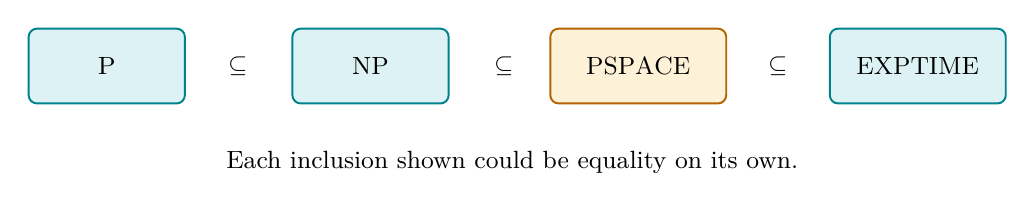
\begin{tikzpicture}[every node/.style={font=\small}]
\node[block,text width=1.75cm] (p) at (0,0) {$\mathrm P$};
\node[block,text width=1.75cm] (np) at (3.35,0) {$\mathrm{NP}$};
\node[amberblock,text width=2cm] (ps) at (6.75,0) {$\mathrm{PSPACE}$};
\node[block,text width=2cm] (ex) at (10.3,0) {$\mathrm{EXPTIME}$};
\node at (1.675,0) {$\subseteq$};
\node at (5.05,0) {$\subseteq$};
\node at (8.525,0) {$\subseteq$};
\node[align=center] at (5.15,-1.22) {Each inclusion shown could be equality on its own.};
\end{tikzpicture}\par
\end{tcolorbox}

\begin{itemize}[leftmargin=*, itemsep=3pt, topsep=4pt]
  \item \textbf{P is contained in NP.} A deterministic polynomial-time algorithm can act as the verifier.
  \item \textbf{NP is contained in PSPACE.} Enumerate all polynomial-length certificates and verify one at a time, reusing the space. The number of certificates may be exponential.
  \item \textbf{PSPACE is contained in EXPTIME.} A deterministic polynomial-space machine has at most exponentially many configurations. A halting run cannot revisit an identical configuration and then continue differently.
  \item \textbf{Completeness.} A problem is PSPACE-complete if it is in PSPACE and every problem in PSPACE reduces to it in polynomial time. A PSPACE-complete problem being in NP would imply $\mathrm{NP}=\mathrm{PSPACE}$.
\end{itemize}
The displayed containments do not resolve which adjacent classes are equal. The time hierarchy theorem does give $\mathrm{P}\subsetneq\mathrm{EXPTIME}$, so at least one adjacent inclusion in the chain is strict.

\subsection{True Quantified Boolean Formula}
\begin{tcolorbox}[defbox, title={TQBF}]
TQBF asks whether a fully quantified Boolean formula is true. An existential quantifier $\exists x$ requires at least one of $x=0,1$ to work. A universal quantifier $\forall x$ requires both to work. The quantifier order determines which choices may depend on earlier ones.
\end{tcolorbox}

\begin{tcolorbox}[examplebox, title={Quantifier order matters}]
The formula $\forall x\,\exists y\,(x\leftrightarrow y)$ is true because the choice $y=x$ works for either value of $x$. The formula $\exists y\,\forall x\,(x\leftrightarrow y)$ is false because a single fixed value of $y$ cannot match both values of $x$.
\end{tcolorbox}

\begin{tcolorbox}[formulabox, title={Depth-first evaluation of a quantified Boolean formula}]
\begin{verbatim}
If there are no quantifiers left, evaluate the matrix.
For an existential variable:
    evaluate assignments 0 and 1 as needed and take OR.
For a universal variable:
    evaluate assignments 0 and 1 as needed and take AND.
Reuse the assignment array after each recursive result.
\end{verbatim}
\end{tcolorbox}

\begin{itemize}[leftmargin=*, itemsep=2pt]
  \item \textbf{Time.} In the worst case the evaluator tries exponentially many assignments.
  \item \textbf{Working space.} The recursion depth is $n$. Store the formula and one partial assignment, and reuse the same storage when trying the next branch.
  \item \textbf{Completeness.} This shows $\mathrm{TQBF}\in\mathrm{PSPACE}$. To prove hardness, encode the reachability question for a polynomial-space machine as a quantified formula. The construction below uses one copy of the smaller reachability test per recursion level.
\end{itemize}

\subsection{Savitch's theorem and the space viewpoint}
\begin{tcolorbox}[formulabox, title={Savitch's theorem}]
For standard space bounds $s(n)\ge\log n$,
\[
\mathrm{NSPACE}(s(n))\subseteq\mathrm{DSPACE}(s(n)^2).
\]
In particular $\mathrm{NPSPACE}=\mathrm{PSPACE}$. This equality is about polynomial space. It does not imply $\mathrm{P}=\mathrm{NP}$.
\end{tcolorbox}

\textbf{Proof idea using reachability.} Let $R(a,b,k)$ mean that configuration $b$ is reachable from $a$ in at most $2^k$ steps.
\begin{enumerate}[leftmargin=*, itemsep=3pt]
  \item \textbf{Base case.} At $k=0$, check whether $a=b$ or a single legal move takes $a$ to $b$.
  \item \textbf{Recursive step.} Try each candidate midpoint $m$. Accept if both $R(a,m,k-1)$ and $R(m,b,k-1)$ hold for the same $m$.
  \item \textbf{Space bound.} Evaluate the two calls in sequence and reuse their storage. There are $2^{O(s)}$ configurations, so $O(s)$ levels suffice. Each level keeps $O(s)$ bits of configurations and counters. Total working space is $O(s^2)$.
\end{enumerate}

\textbf{Readings.} \href{https://ocw.mit.edu/courses/6-046j-design-and-analysis-of-algorithms-spring-2015/pages/lecture-notes/}{MIT 6.046J lecture notes on randomization and approximation}. Walter J. Savitch, \href{https://doi.org/10.1016/S0022-0000(70)80006-X}{Relationships Between Nondeterministic and Deterministic Tape Complexities (1970)}.

\subsection{How a quantified formula encodes reachability}
A configuration records a machine's state, head positions and working tape. For a polynomial-space machine, that record uses a polynomial number of bits $m$.

\begin{enumerate}[leftmargin=*, itemsep=3pt]
  \item \textbf{Encode one move.} The formula $R_0(x,y)$ checks whether the configurations are identical or one legal step connects them. The legal-step test has polynomial size because it checks the local update and the unchanged parts.
  \item \textbf{Check both halves with one formula.} Guess a midpoint $z$. Fresh universally quantified vectors $u,v$ select the pairs $(x,z)$ and $(z,y)$.
  \[
  \begin{aligned}
  R_k(x,y)={}&\exists z\,\forall u\,\forall v\,\big[
    \big((u=x\land v=z)\lor(u=z\land v=y)\big)\\
    &\hspace{8em}\Longrightarrow R_{k-1}(u,v)\big].
  \end{aligned}
  \]
  The antecedent is true for the two selected pairs, so each smaller reachability test must pass. For every other pair the implication is true automatically.
  \item \textbf{Bound the construction.} There are at most $2^m$ encoded configurations, so $k=m$ suffices. Each level adds polynomially many symbols and uses only one copy of $R_{k-1}$. The full formula is therefore polynomial in length.
  \item \textbf{Set the endpoints.} Start at the machine's initial configuration and existentially choose an accepting target. The formula is true exactly when the machine accepts.
\end{enumerate}

\textbf{Further reading.} \href{https://ocw.mit.edu/courses/18-404j-theory-of-computation-fall-2020/resources/lecture-18-pspace-completeness/}{MIT 18.404J lecture on PSPACE-completeness}.

\newpage
\begin{center}
  {\large\bfseries\color{myred} Quick Revision --- Module 5}\\[3pt]
  {\small\color{mydark} Approximation, Randomization and PSPACE $|$ ES-CS401}
\end{center}
\noindent{\color{myred}\rule{\linewidth}{1.2pt}}\par\vspace{4pt}

\begin{tcolorbox}[formulabox, title={Key Concepts at a Glance}]
\renewcommand{\arraystretch}{1.35}
\noindent\begin{tabularx}{\linewidth}{B{4.5cm}Y}
Minimisation ratio & $A\le\rho\,\mathrm{OPT}$ for all supported inputs. \\[3pt]
Maximisation ratio & $A\ge\mathrm{OPT}/\rho$. \\[3pt]
Matching lower bound & $\mathrm{OPT}_{\mathrm{VC}}\ge|M|$ for any matching $M$. \\[3pt]
One-sided repetition & At most $p^k$ error after $k$ independent trials under the appropriate acceptance rule. \\[3pt]
Space inclusions & $\mathrm P\subseteq\mathrm{NP}\subseteq\mathrm{PSPACE}\subseteq\mathrm{EXPTIME}$. \\[3pt]
\end{tabularx}\par
\end{tcolorbox}

\begin{tcolorbox}[defbox, title={One-Line Definitions}]
\begin{itemize}[leftmargin=*, itemsep=3pt, topsep=4pt]
  \item \textbf{Approximation ratio.} A proved factor relating feasible objective value to the optimum.
  \item \textbf{Las Vegas algorithm.} A randomized procedure with exact answers and variable running time.
  \item \textbf{Monte Carlo algorithm.} A bounded-time randomized procedure with a stated error probability.
  \item \textbf{PSPACE.} Decision problems solvable using polynomial working space.
\end{itemize}
\end{tcolorbox}

\begin{tcolorbox}[exambox, title={Frequently Asked / Viva Questions}]
\begin{enumerate}[topsep=0pt, label=\textbf{Q\arabic*.}, itemsep=5pt, leftmargin=*]
  \item \Q{What separates a heuristic from an approximation algorithm?}
    An approximation algorithm proves a solution-quality guarantee for a stated problem family.
  \item \Q{What is special about an FPTAS?}
    Its runtime is polynomial in input length and in $1/\varepsilon$.
  \item \Q{Why does the cover algorithm use a matching?}
    Each selected disjoint edge contributes a separate mandatory endpoint to any cover.
  \item \Q{Which assumption justifies shortcutting the metric TSP traversal?}
    The triangle inequality bounds the shortcut by the path it replaces.
  \item \Q{How can a randomized algorithm have worst-case and expected bounds?}
    Worst case considers the unluckiest choices. Expectation averages over the algorithm's own random choices on a fixed input.
  \item \Q{What is the worst-case time for random-pivot quicksort?}
    $\Theta(n^2)$ when each pivot is an extreme key.
  \item \Q{What is the error direction of the matrix product test?}
    It can accept a false product. A correct product always passes.
  \item \Q{Why is NP contained in PSPACE?}
    Verify polynomial-length certificates one at a time and reuse the work tape.
  \item \Q{Why can TQBF be evaluated in polynomial space?}
    A depth-first evaluation stores only the current partial assignment and recursion state.
  \item \Q{What does Savitch's theorem prove for polynomial space?}
    $\mathrm{NPSPACE}=\mathrm{PSPACE}$.
  \item \Q{Does the inclusion chain settle P versus NP?}
    The equality question remains open.
\end{enumerate}
\end{tcolorbox}

\begin{tcolorbox}[tikzbox, title={Summary Comparison}]
\par\vspace{5pt}
\begingroup
\setlength{\extrarowheight}{1pt}
\noindent\begin{tabularx}{\linewidth}{|B{3.45cm}|Y|Y|}
\hline
\textbf{Topic} & \textbf{Main goal} & \textbf{Standard example} \\ \hline
Approximation & Guaranteed feasible quality in polynomial time. & Maximal-matching vertex cover. \\ \hline
Las Vegas & Always correct with expected resource bounds. & Random-pivot quicksort. \\ \hline
Monte Carlo & Fast test with controlled error. & Freivalds' matrix product check. \\ \hline
Polynomial space & Reuse memory across an extensive search. & Depth-first TQBF evaluation. \\ \hline
\end{tabularx}\par
\endgroup
\end{tcolorbox}


\end{document}
